\documentclass[aspectratio=169]{beamer}

\usepackage{animate}
\usepackage{booktabs}
\setbeamertemplate{caption}[numbered]
\setbeamertemplate{footline}[frame number]
\setbeamertemplate{navigation symbols}{}

\usepackage{amsmath}
\newcommand*{\norm}[1]{\left\lVert#1\right\rVert}
\newcommand{\argmin}{\arg\!\min}

\usepackage{color,soul}
\usepackage{colortbl}
\usepackage{graphicx}

\setbeamerfont{footnote}{size=\tiny}

\usepackage{listings,lstautogobble}
\lstset{language=Python,
	basicstyle=\scriptsize\ttfamily,
	commentstyle=\ttfamily\itshape\color{gray},
	showstringspaces=false,
	autogobble=true
}

\usepackage{caption}
\captionsetup{justification=centering,margin=1cm}
\usepackage{subcaption}

\usepackage{multirow}
\usepackage{nicematrix}
\NiceMatrixOptions{
	code-for-first-row=\color{blue},
	code-for-first-col=\color{blue}
}

\usepackage{pifont}% http://ctan.org/pkg/pifont
\newcommand{\cmark}{\ding{51}}%
\newcommand{\xmark}{\ding{55}}%

\usepackage{siunitx}
\usepackage{tikz}
\tikzstyle{process} = [rectangle, minimum width=3cm, minimum height=1cm, text centered, draw=black, fill=orange!30]
\usetikzlibrary{shapes,positioning}
\usepackage{ulem}

\AtBeginSection[]{
	\begin{frame}
		\vfill
		\centering
		\begin{beamercolorbox}[sep=8pt,center,shadow=true,rounded=true]{title}
			\usebeamerfont{title}\insertsectionhead\par%
		\end{beamercolorbox}
		\vfill
	\end{frame}
}

\addtobeamertemplate{footnote}{\hskip -2em}{}

\usepackage[capitalise,noabbrev]{cleveref}
\usepackage[numbers,sort&compress]{natbib}
\bibliographystyle{unsrt}

\usepackage{xcolor}
\usepackage{hyperref}
\hypersetup{
	colorlinks=true,
	linkcolor=blue,  % color for internal links
	urlcolor=cyan   % color for external links
}

\setbeamercolor{block title}{fg=black,bg=yellow}
\setbeamertemplate{blocks}[rounded][shadow]
\setbeamerfont{block body}{size=\scriptsize}
\setbeamerfont{block title example}{size=\tiny}

\title{Image Reconstruction 2: \\
Compressed Sensing \& Low-Rank Models}
\author{Zhengguo Tan, Ph.D.}
\institute{Michigan Institute for Imaging Technology and Translation (MIITT) \\
	University of Michigan, Ann Arbor, Michigan, USA}
\date{September 30, 2025}

\logo{
\includegraphics[width=.16\textwidth]{figures/um.png}\vspace*{0.82\paperheight}}

\begin{document}
	\frame{\titlepage}
	\logo{}  % make logo appear only in the title page
	
	\begin{frame}
		\frametitle{Outline}
		\tableofcontents
	\end{frame}
	
	% ============================================ %
	\section{Funny Intro to Compressed Sensing}
	
	\begin{frame}{Compressed Sensing: Definition}
		\begin{columns}
			\column{0.6\textwidth}
			\centering
			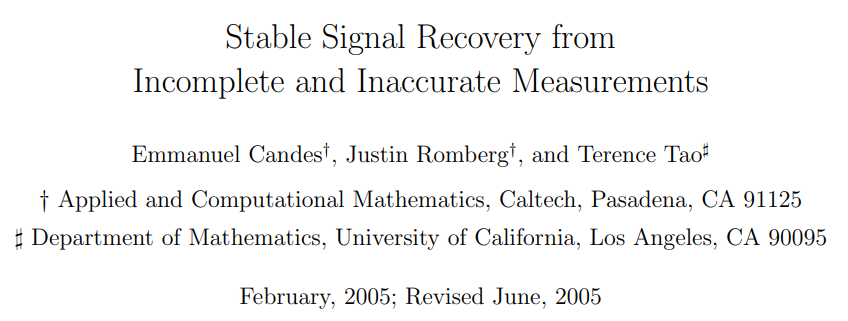
\includegraphics[width=\columnwidth]{figures/cs-01.png}
			
			\begin{equation}
				\text{min} \norm{x}_{\ell_1} \;\; \text{subject to} \norm{A x - y}_{\ell_2} \leq \epsilon
			\end{equation}
			
			\begin{equation}
				\argmin_x \norm{A x - y}_2 + \lambda \norm{R x}_1
			\end{equation}
			
			\column{0.4\textwidth}
			\centering
			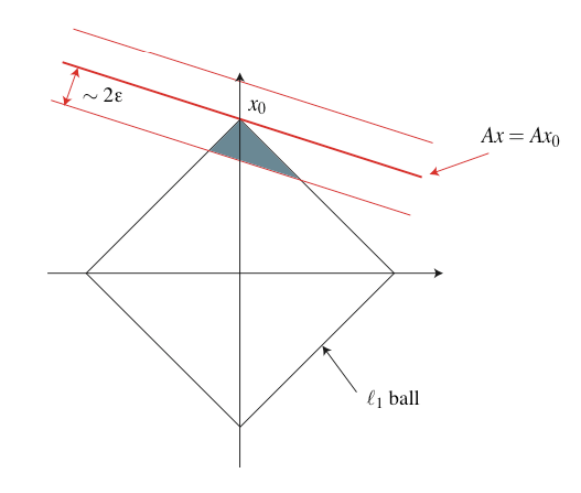
\includegraphics[width=\columnwidth]{figures/cs-02.png}
		\end{columns}
	\end{frame}
	
	\begin{frame}{Compressed Sensing MRI}
		\begin{figure}
			\centering
			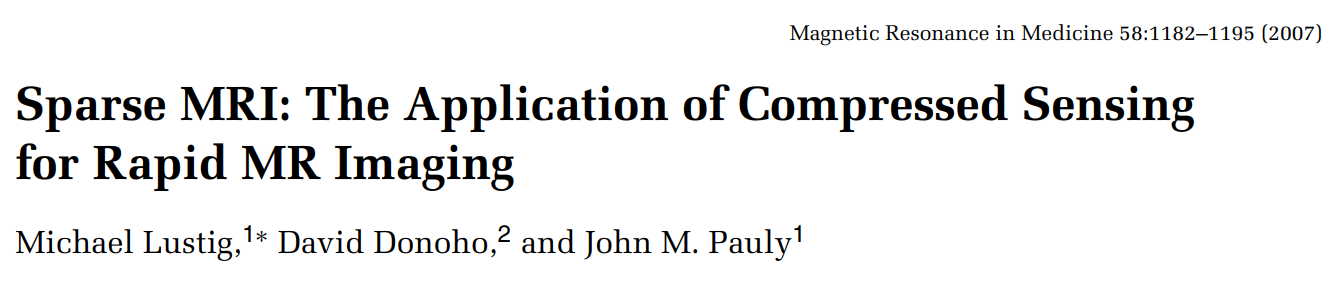
\includegraphics[width=\textwidth]{figures/cs-lustig.png}
		\end{figure}
	\end{frame}
	
	\begin{frame}{Compressed Sensing: Funny Intro from Miki Lustig}
		Source: \url{https://people.eecs.berkeley.edu/~mlustig/comics0.html}
		\vspace{1em}
		\begin{columns}
			\column{0.5\textwidth}
			\centering
			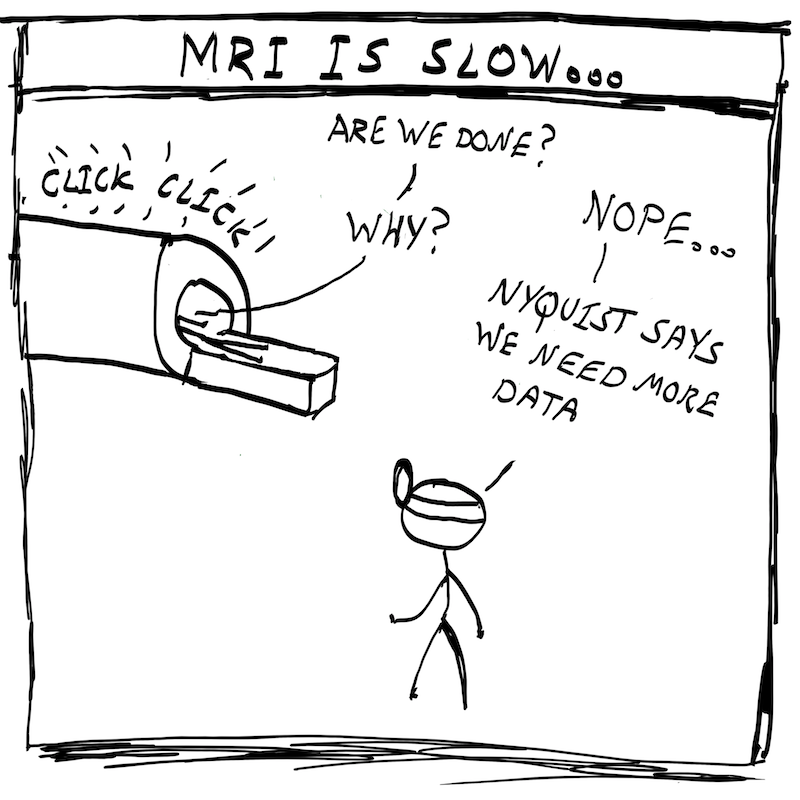
\includegraphics[width=\columnwidth]{figures/cs-lustig-comics-01.png}
			
			\column{0.5\textwidth}
			\centering
			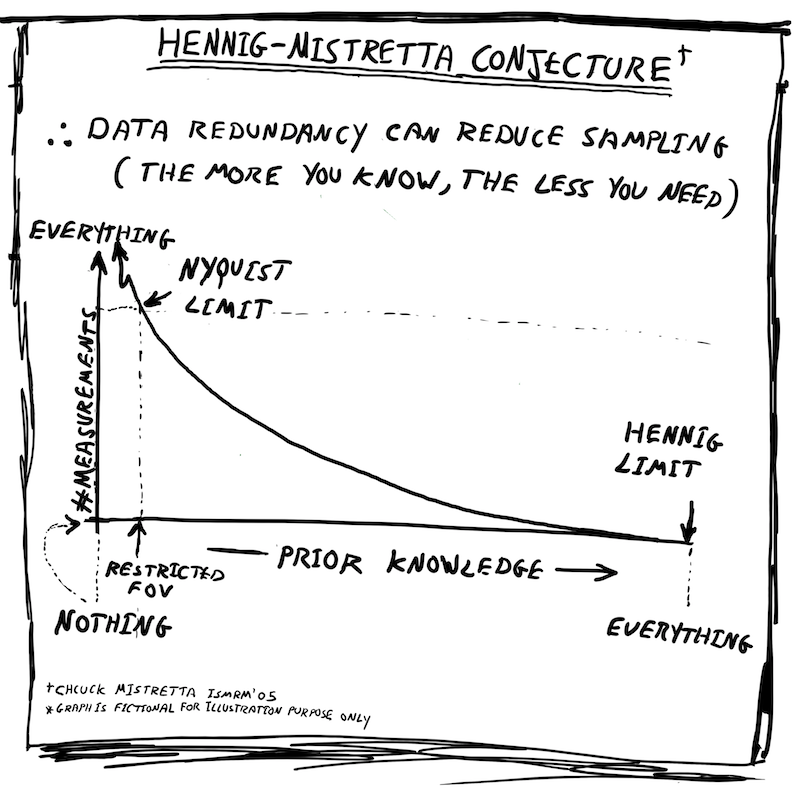
\includegraphics[width=\columnwidth]{figures/cs-lustig-comics-02.png}
		\end{columns}
	\end{frame}
	
	\begin{frame}{Compressed Sensing: Funny Intro from Miki Lustig}
		Source: \url{https://people.eecs.berkeley.edu/~mlustig/comics0.html}
		\vspace{1em}
		\begin{columns}
			\column{0.5\textwidth}
			\centering
			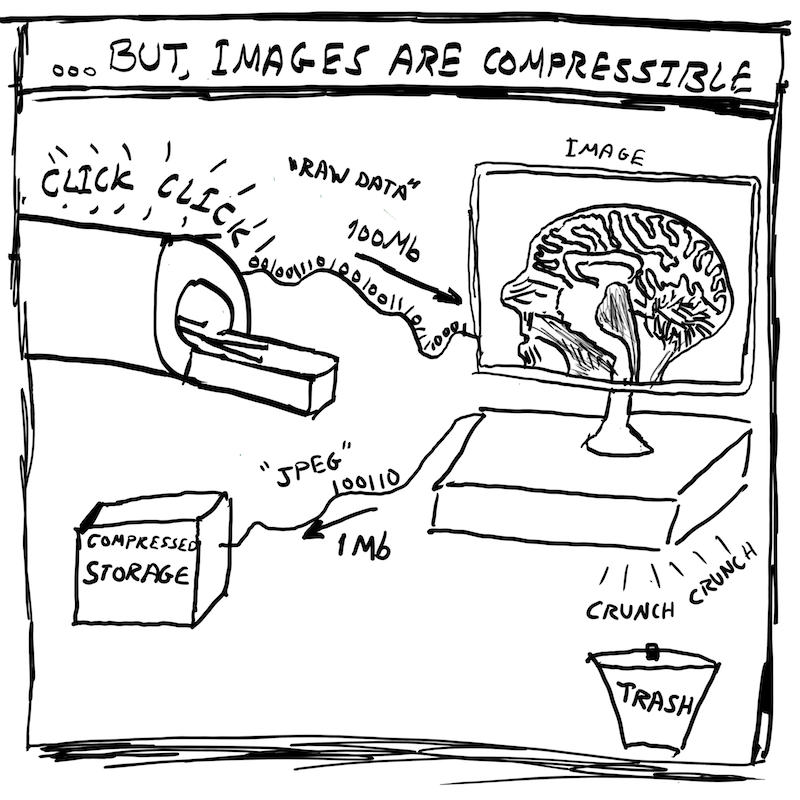
\includegraphics[width=\columnwidth]{figures/cs-lustig-comics-03.png}
			
			\column{0.5\textwidth}
			\centering
			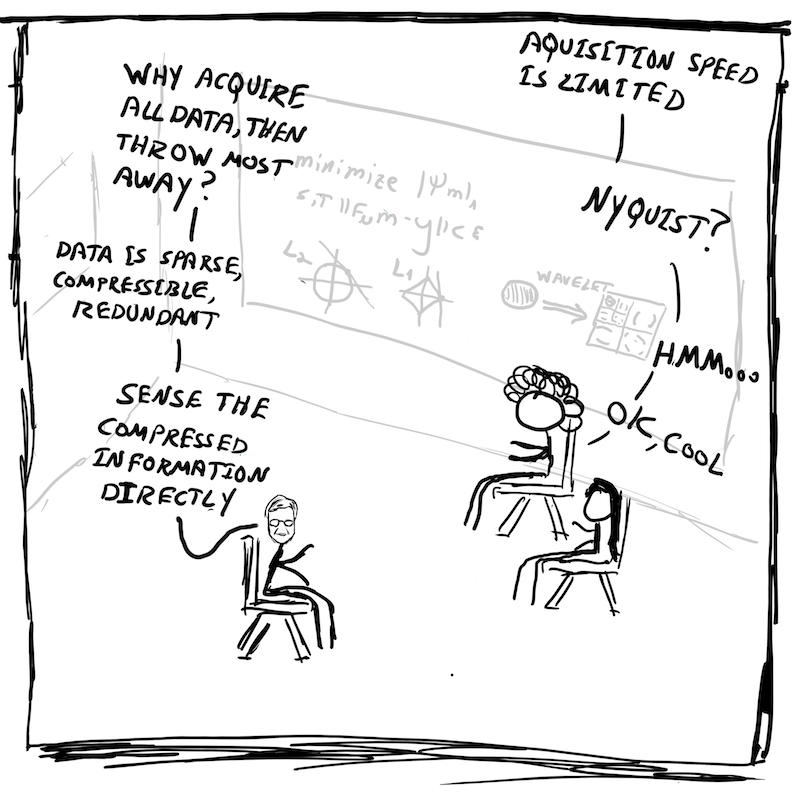
\includegraphics[width=\columnwidth]{figures/cs-lustig-comics-04.png}
		\end{columns}
	\end{frame}
	
	\begin{frame}{Compressed Sensing: Funny Intro from Miki Lustig}
		Source: \url{https://people.eecs.berkeley.edu/~mlustig/comics0.html}
		\vspace{1em}
		\begin{columns}
			\column{0.5\textwidth}
			\centering
			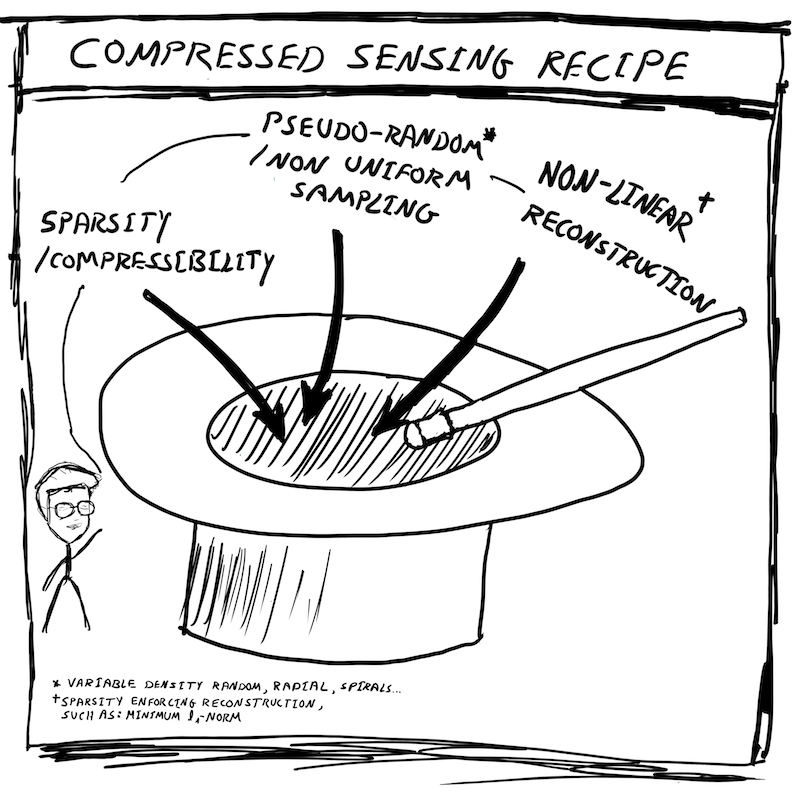
\includegraphics[width=\columnwidth]{figures/cs-lustig-comics-05.png}
			
			\column{0.5\textwidth}
			\centering
			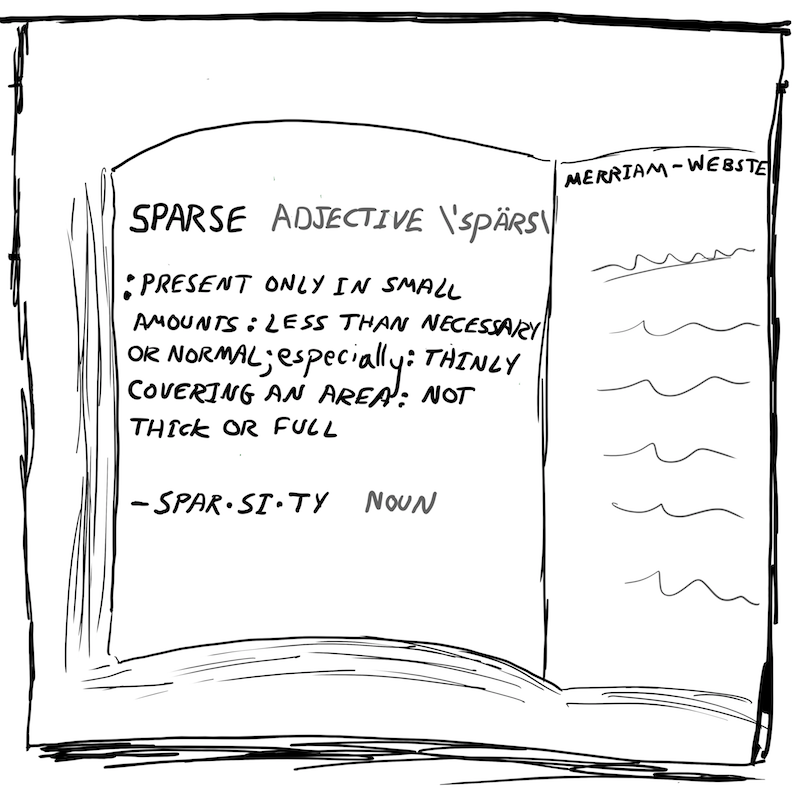
\includegraphics[width=\columnwidth]{figures/cs-lustig-comics-06.png}
		\end{columns}
	\end{frame}
	
	\begin{frame}{Compressed Sensing: Funny Intro from Miki Lustig}
		Source: \url{https://people.eecs.berkeley.edu/~mlustig/comics0.html}
		\vspace{1em}
		\begin{columns}
			\column{0.5\textwidth}
			\centering
			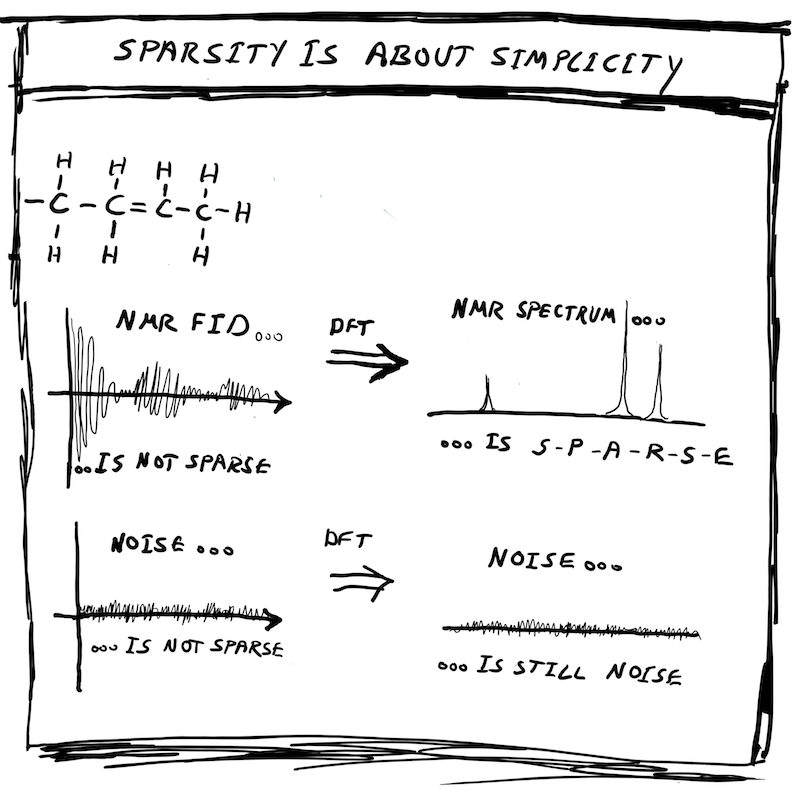
\includegraphics[width=\columnwidth]{figures/cs-lustig-comics-07.png}
			
			\column{0.5\textwidth}
			\centering
			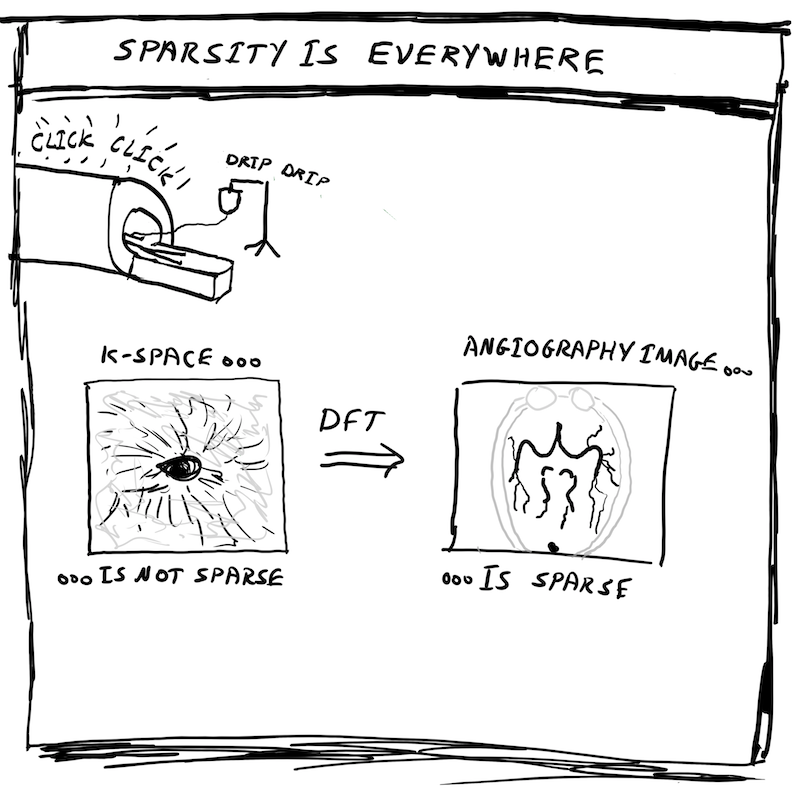
\includegraphics[width=\columnwidth]{figures/cs-lustig-comics-08.png}
		\end{columns}
	\end{frame}
	
	\begin{frame}{Compressed Sensing: Funny Intro from Miki Lustig}
		Source: \url{https://people.eecs.berkeley.edu/~mlustig/comics0.html}
		\vspace{1em}
		\begin{columns}
			\column{0.5\textwidth}
			\centering
			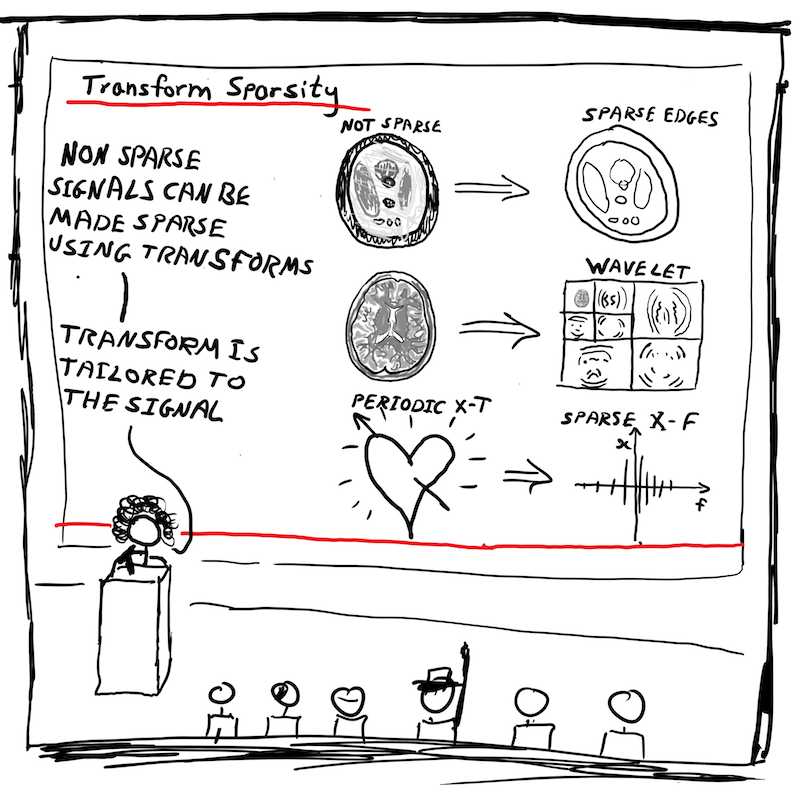
\includegraphics[width=\columnwidth]{figures/cs-lustig-comics-09.png}
			
			\column{0.5\textwidth}
			\centering
			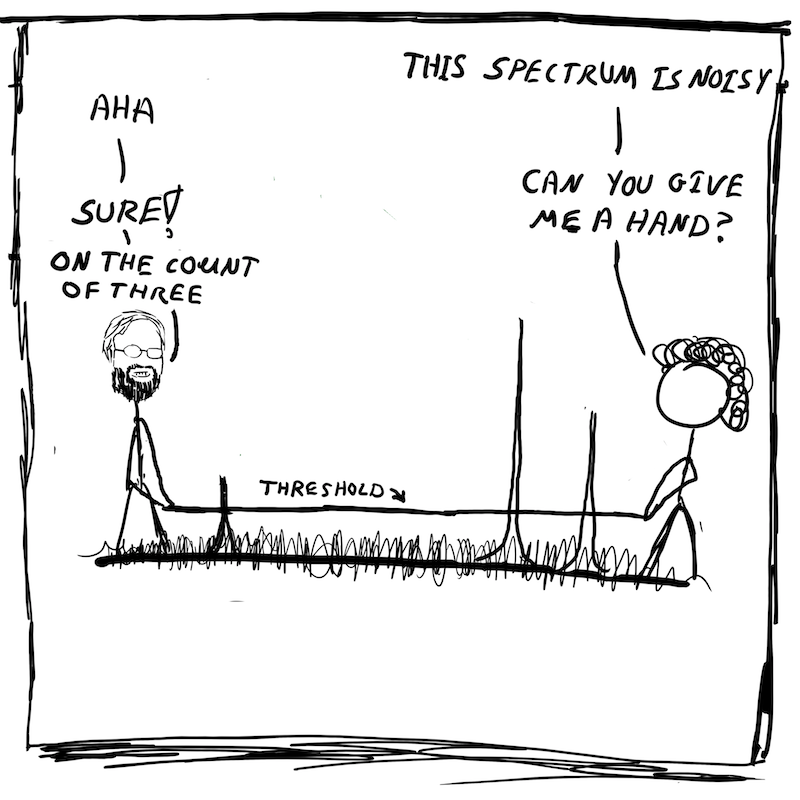
\includegraphics[width=\columnwidth]{figures/cs-lustig-comics-10.png}
		\end{columns}
	\end{frame}
	
	\begin{frame}{Compressed Sensing: Funny Intro from Miki Lustig}
		Source: \url{https://people.eecs.berkeley.edu/~mlustig/comics0.html}
		\vspace{1em}
		\begin{columns}
			\column{0.5\textwidth}
			\centering
			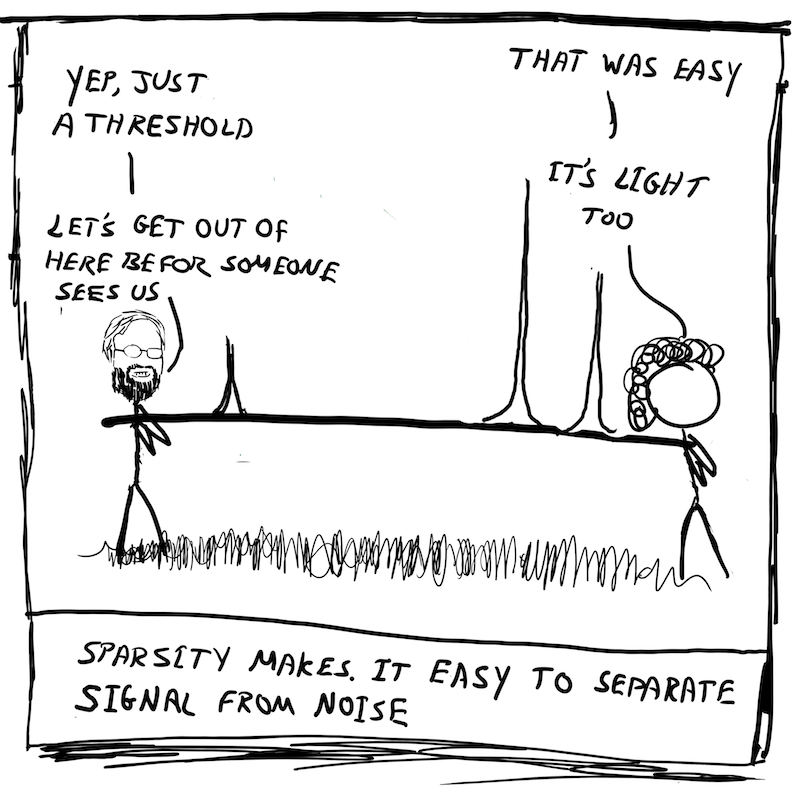
\includegraphics[width=\columnwidth]{figures/cs-lustig-comics-11.png}
			
			\column{0.5\textwidth}
			\centering
			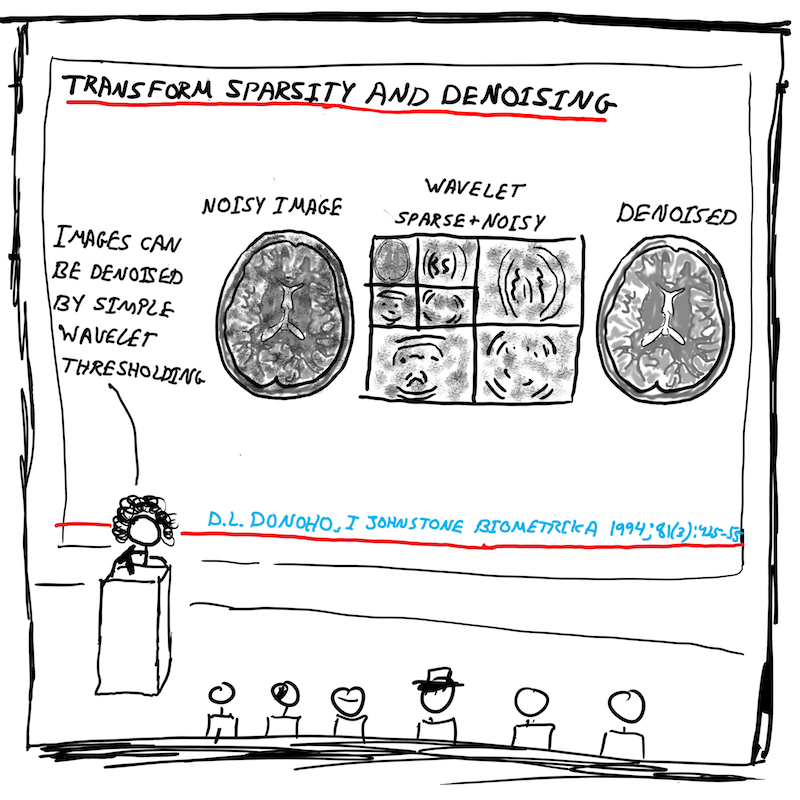
\includegraphics[width=\columnwidth]{figures/cs-lustig-comics-12.png}
		\end{columns}
	\end{frame}
	
	\begin{frame}{Compressed Sensing: Funny Intro from Miki Lustig}
		Source: \url{https://people.eecs.berkeley.edu/~mlustig/comics0.html}
		\vspace{1em}
		\begin{columns}
			\column{0.5\textwidth}
			\centering
			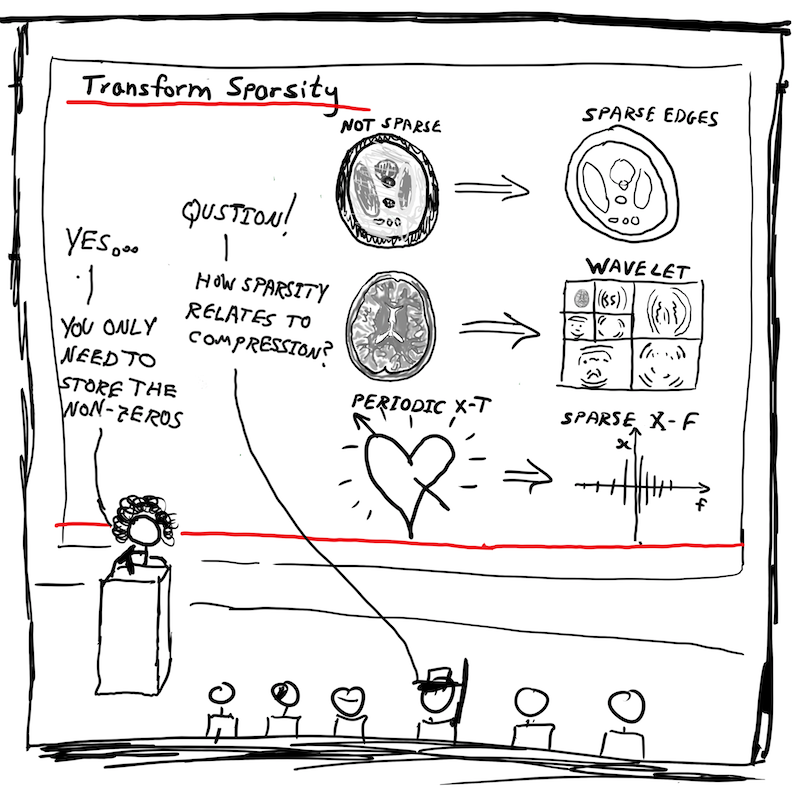
\includegraphics[width=\columnwidth]{figures/cs-lustig-comics-13.png}
			
			\column{0.5\textwidth}
			\centering
			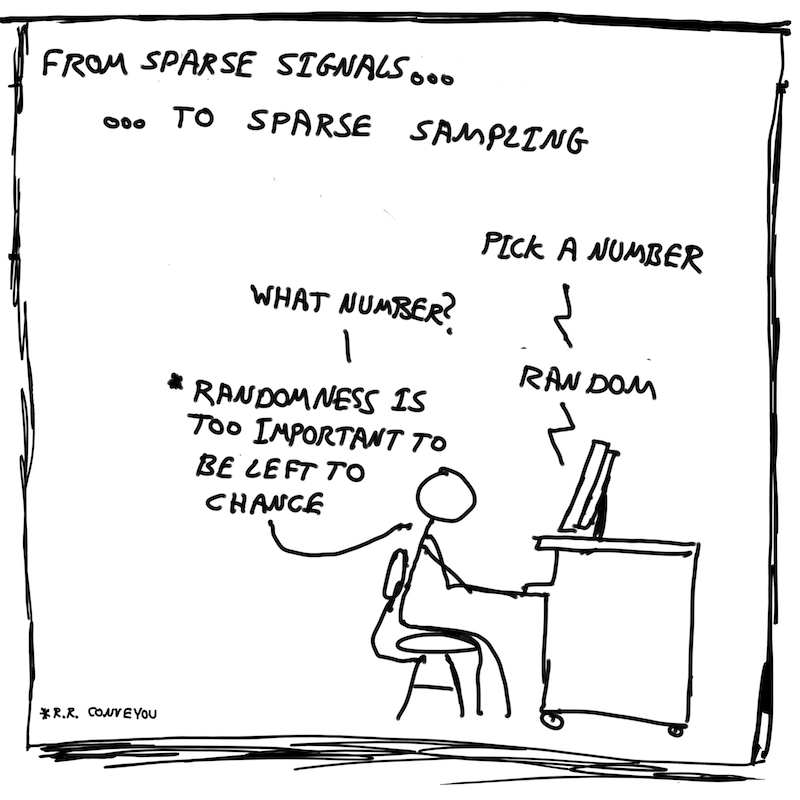
\includegraphics[width=\columnwidth]{figures/cs-lustig-comics-14.png}
		\end{columns}
	\end{frame}
	
	\begin{frame}{Compressed Sensing: Funny Intro from Miki Lustig}
		Source: \url{https://people.eecs.berkeley.edu/~mlustig/comics0.html}
		\vspace{1em}
		\begin{columns}
			\column{0.5\textwidth}
			\centering
			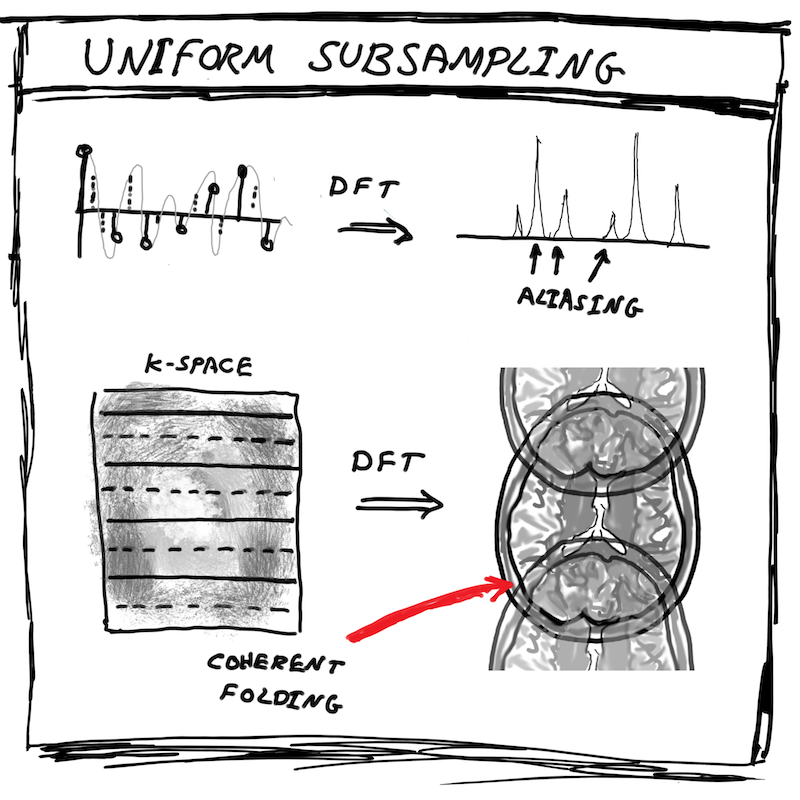
\includegraphics[width=\columnwidth]{figures/cs-lustig-comics-15.png}
			
			\column{0.5\textwidth}
			\centering
			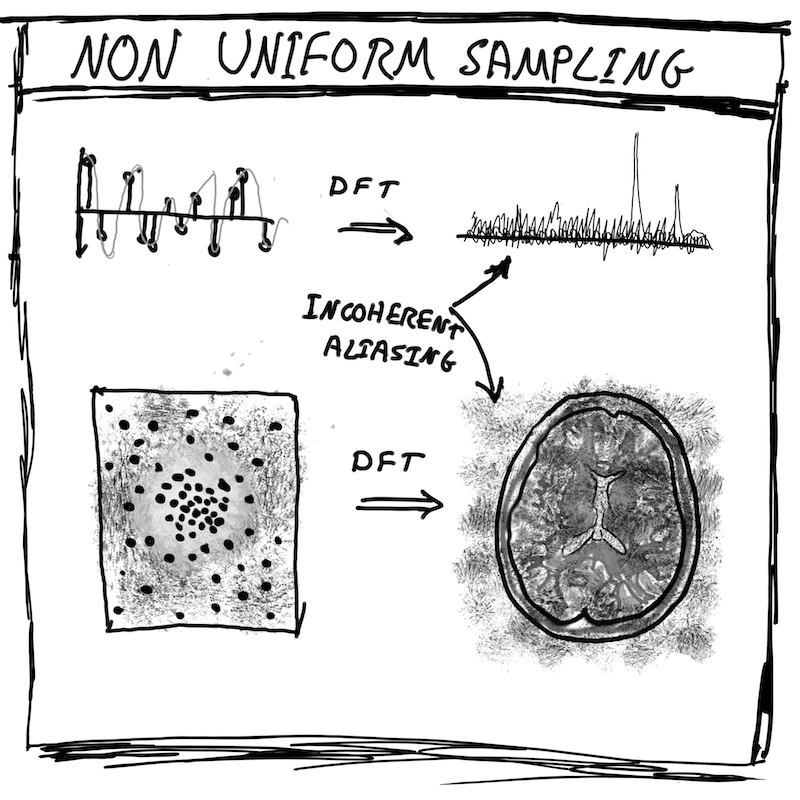
\includegraphics[width=\columnwidth]{figures/cs-lustig-comics-16.png}
		\end{columns}
	\end{frame}
	
	\begin{frame}{Compressed Sensing: Funny Intro from Miki Lustig}
		Source: \url{https://people.eecs.berkeley.edu/~mlustig/comics0.html}
		\vspace{1em}
		\begin{columns}
			\column{0.5\textwidth}
			\centering
			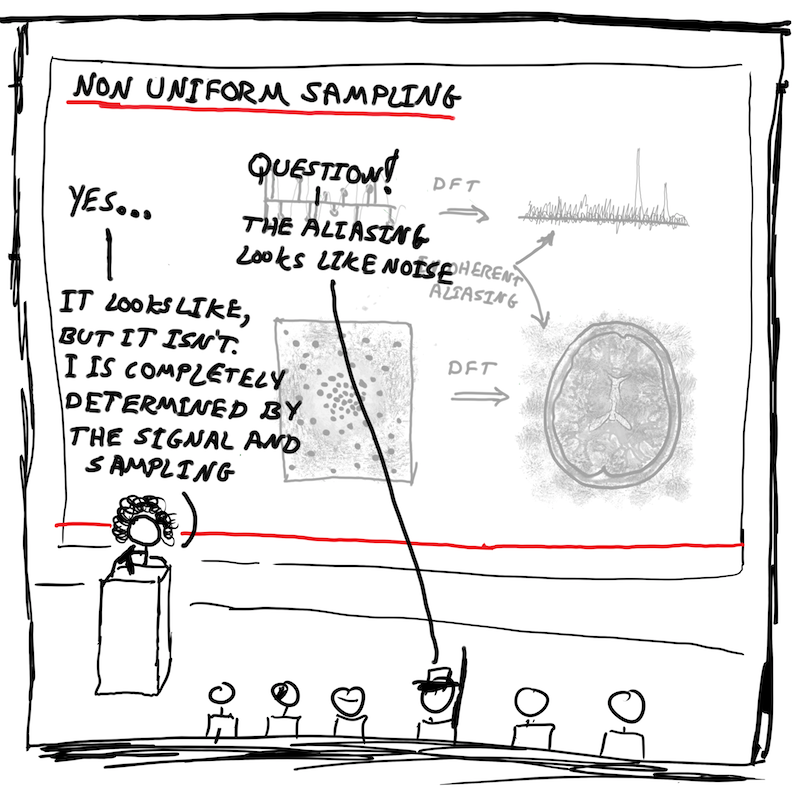
\includegraphics[width=\columnwidth]{figures/cs-lustig-comics-17.png}
			
			\column{0.5\textwidth}
			\centering
			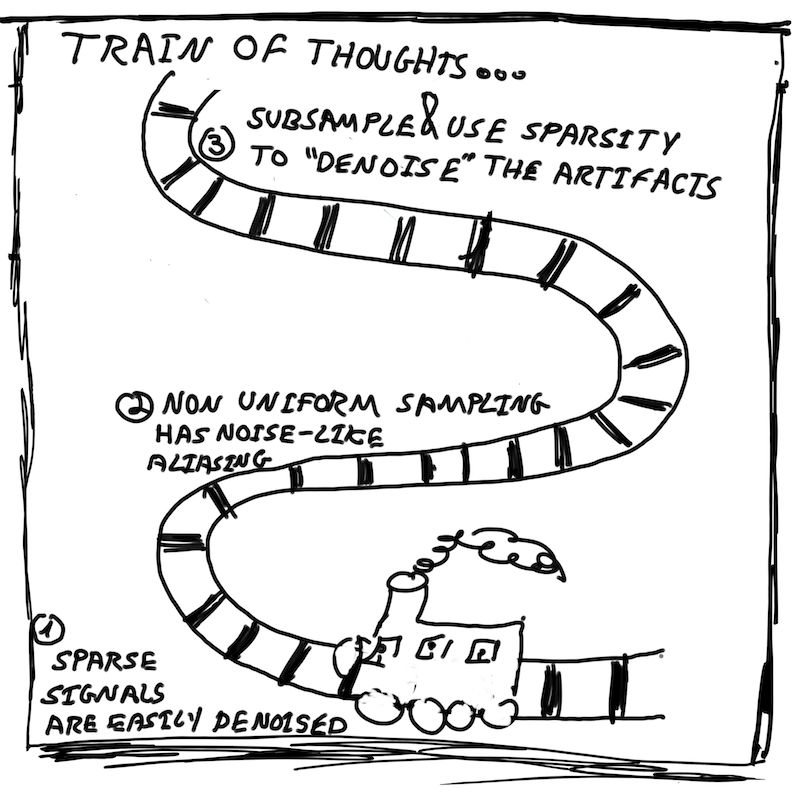
\includegraphics[width=\columnwidth]{figures/cs-lustig-comics-18.png}
		\end{columns}
	\end{frame}
	
	\begin{frame}{Compressed Sensing: Funny Intro from Miki Lustig}
		Source: \url{https://people.eecs.berkeley.edu/~mlustig/comics0.html}
		\vspace{1em}
		\begin{columns}
			\column{0.5\textwidth}
			\centering
			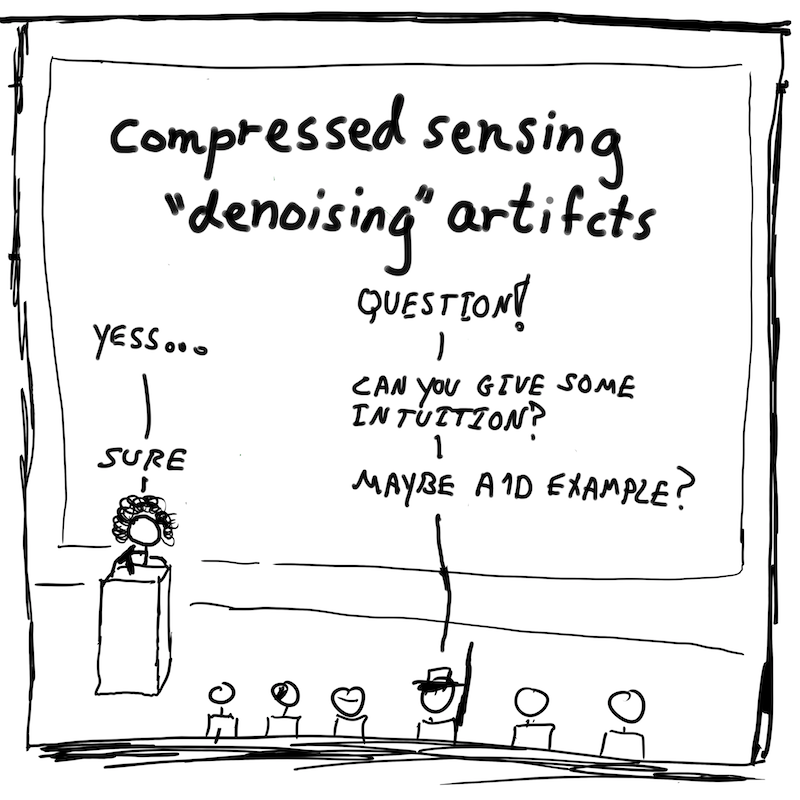
\includegraphics[width=\columnwidth]{figures/cs-lustig-comics-19.png}
			
			\column{0.5\textwidth}
			\centering
			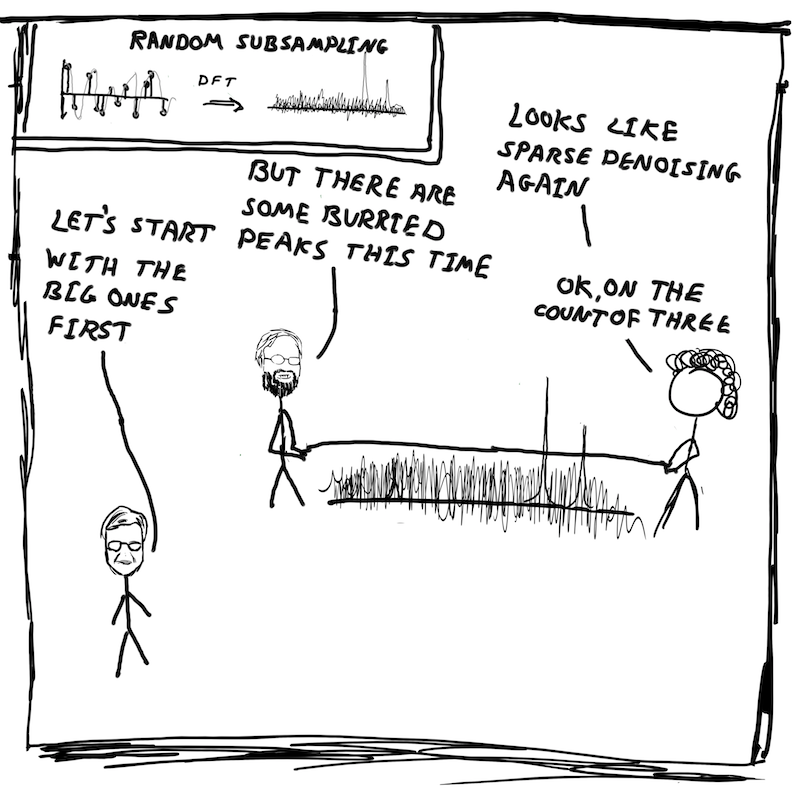
\includegraphics[width=\columnwidth]{figures/cs-lustig-comics-20.png}
		\end{columns}
	\end{frame}
	
	\begin{frame}{Compressed Sensing: Funny Intro from Miki Lustig}
		Source: \url{https://people.eecs.berkeley.edu/~mlustig/comics0.html}
		\vspace{1em}
		\begin{columns}
			\column{0.5\textwidth}
			\centering
			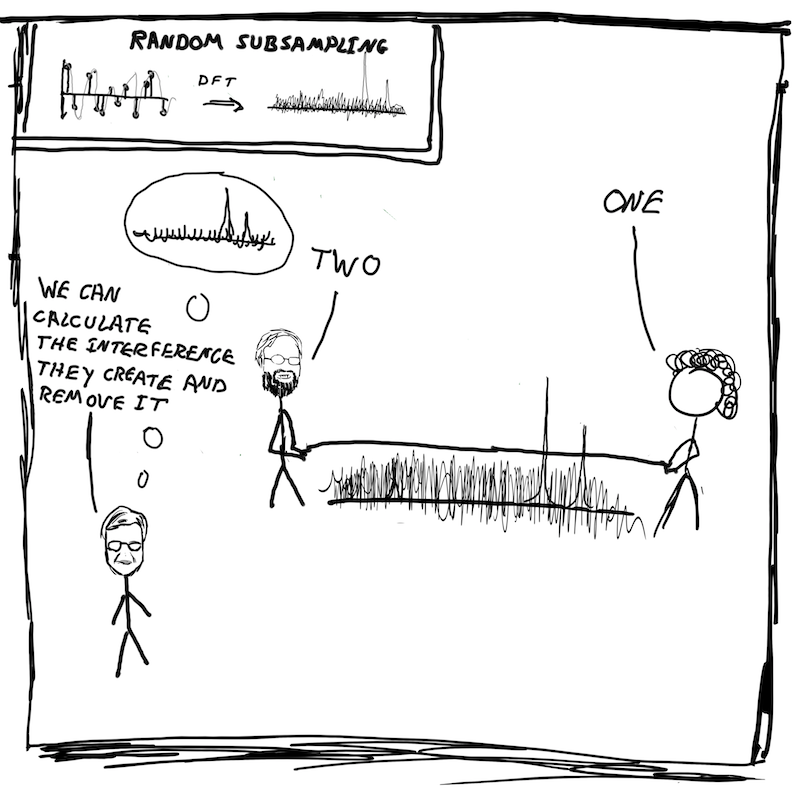
\includegraphics[width=\columnwidth]{figures/cs-lustig-comics-21.png}
			
			\column{0.5\textwidth}
			\centering
			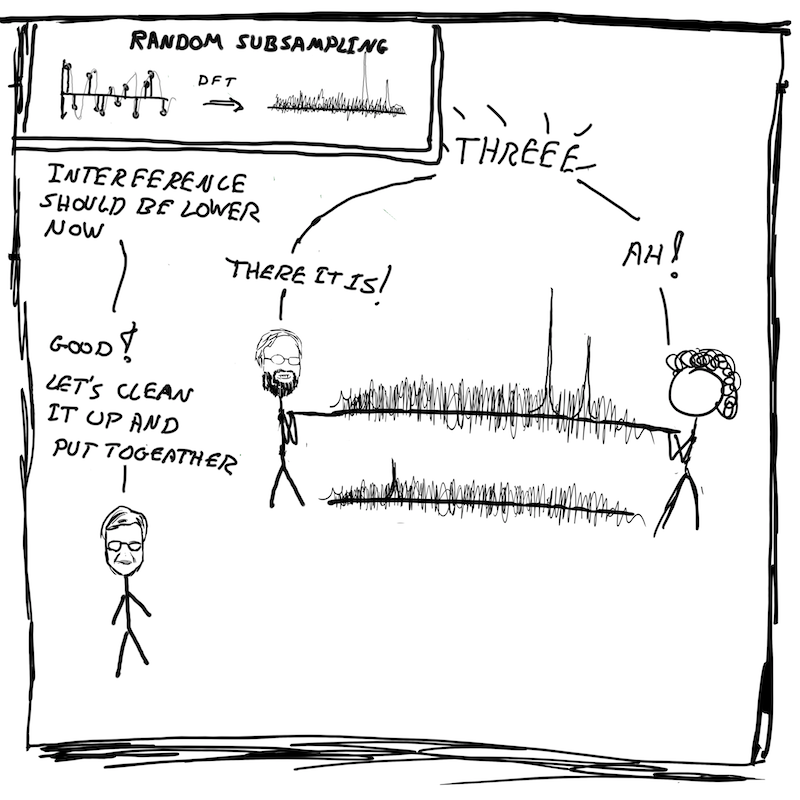
\includegraphics[width=\columnwidth]{figures/cs-lustig-comics-22.png}
		\end{columns}
	\end{frame}
	
	\begin{frame}{Compressed Sensing: Funny Intro from Miki Lustig}
		Source: \url{https://people.eecs.berkeley.edu/~mlustig/comics0.html}
		\vspace{1em}
		\begin{columns}
			\column{0.5\textwidth}
			\centering
			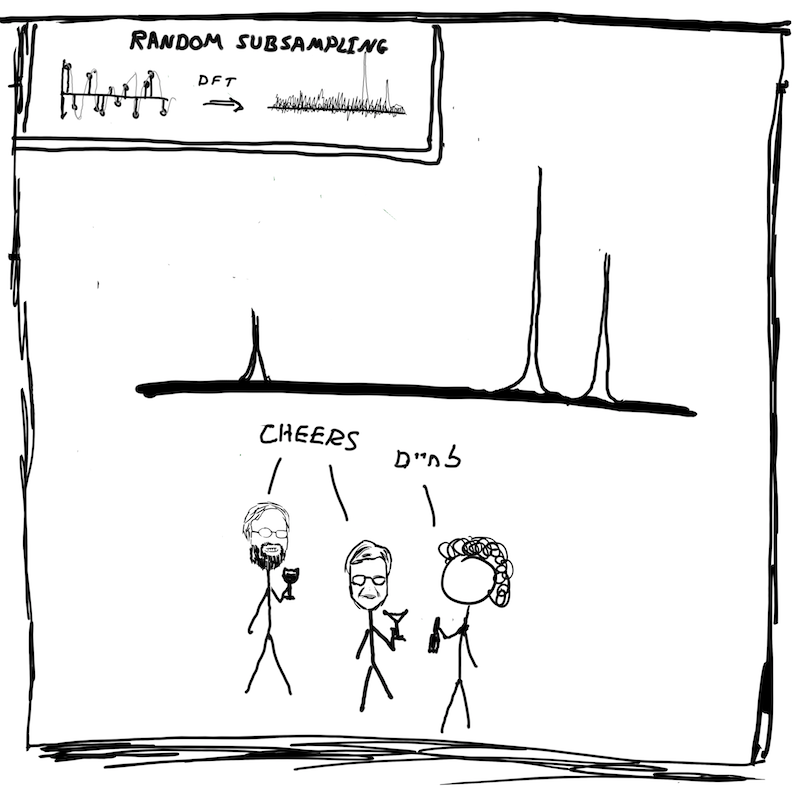
\includegraphics[width=\columnwidth]{figures/cs-lustig-comics-23.png}
			
			\column{0.5\textwidth}
			\centering
			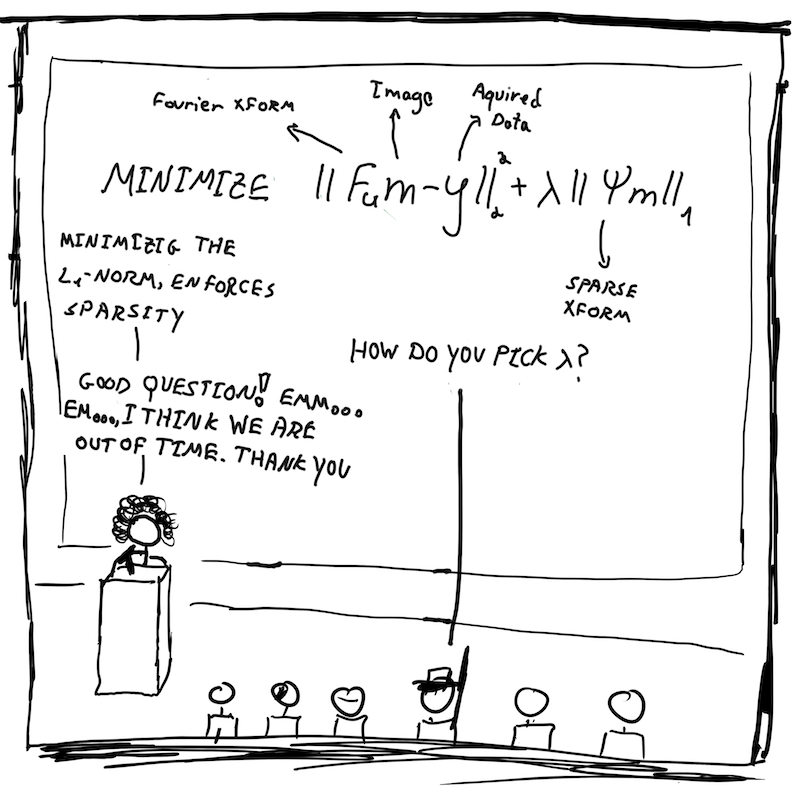
\includegraphics[width=\columnwidth]{figures/cs-lustig-comics-24.png}
		\end{columns}
	\end{frame}
	
	% ============================================ %
	\section{Compressed Sensing}
	
	\begin{frame}{Ingredients in Compressed Sensing}
		
		\begin{enumerate}
			\item Sparsity
			
			\vspace{1em}
			
			\item Incoherence: Non-uniform sampling
			
			\vspace{1em}
			
			\item Non-linear reconstruction
			
		\end{enumerate}
		
	\end{frame}
	
	\begin{frame}{Examples of Sparsity Transform: Wavelet \& Total Variation}
		\begin{columns}
			\column{0.5\textwidth}
			\centering
			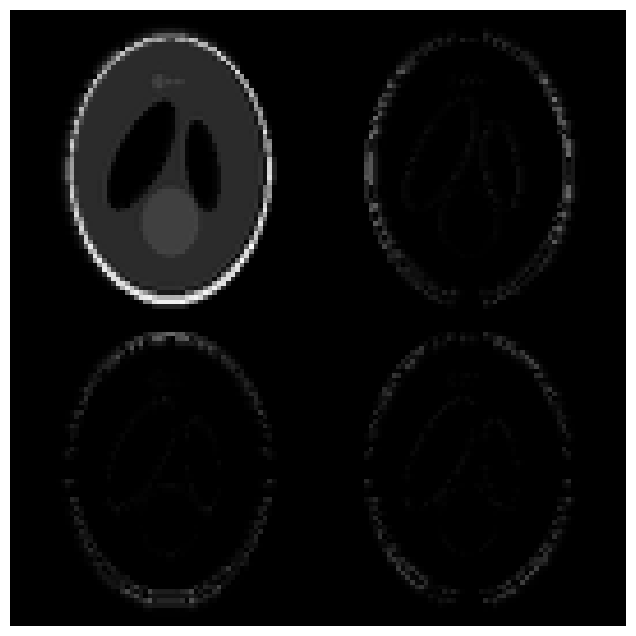
\includegraphics[width=\columnwidth]{figures/spatial_wavelet.png}
			
			\column{0.5\textwidth}
			\centering
			
\includegraphics[width=\columnwidth]{figures/spatial_tv.png}
		\end{columns}
	\end{frame}
	
	\begin{frame}{Uniform Undersampling}
		\begin{figure}
			\centering
			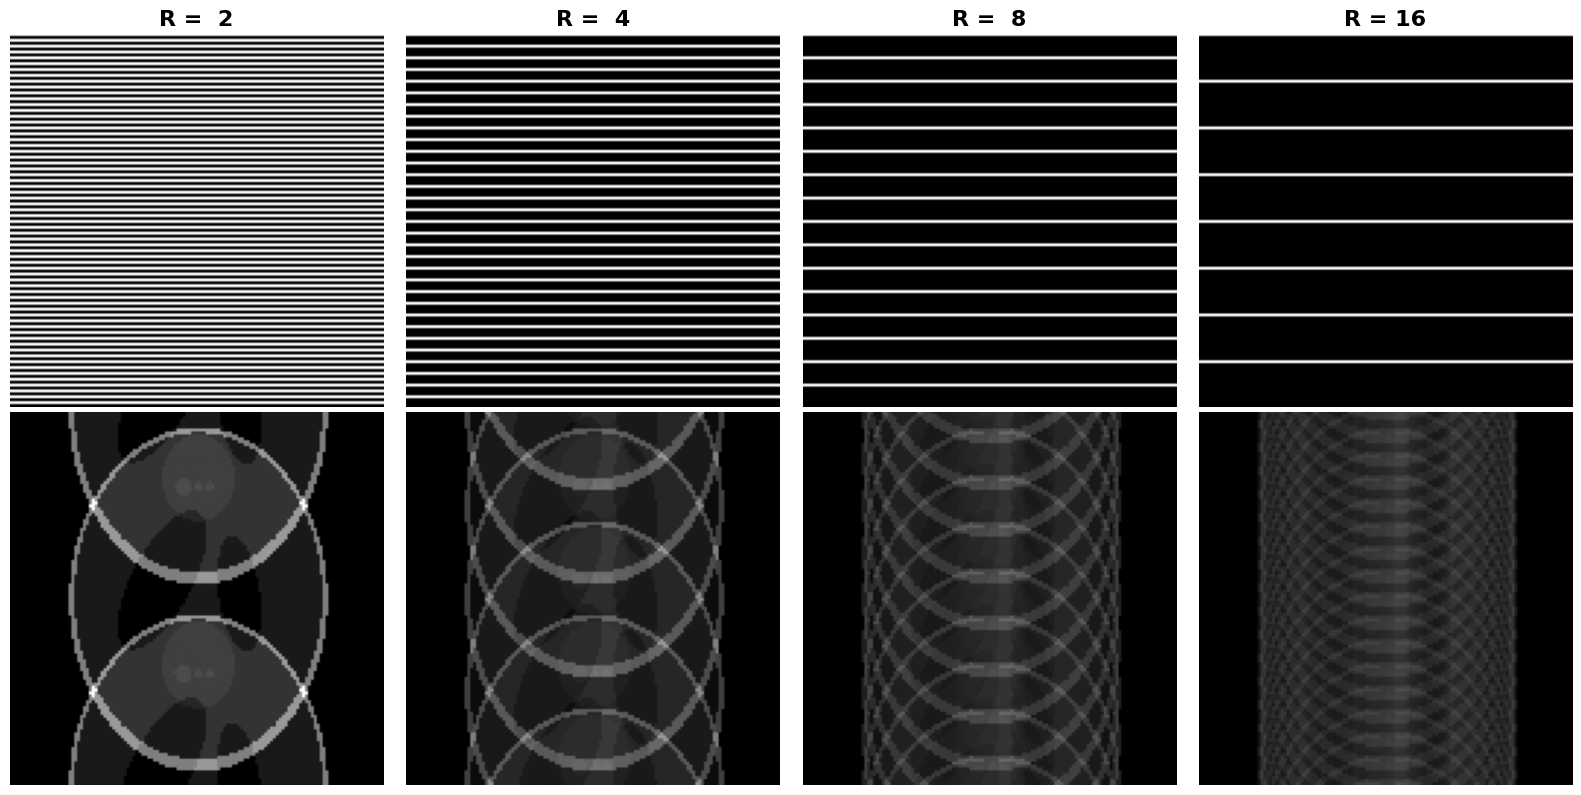
\includegraphics[width=\textwidth]{figures/usamp_cartes.png}
		\end{figure}
	\end{frame}
	
	\begin{frame}{Non-Uniform Undersampling: Poisson}
		\begin{figure}
			\centering
			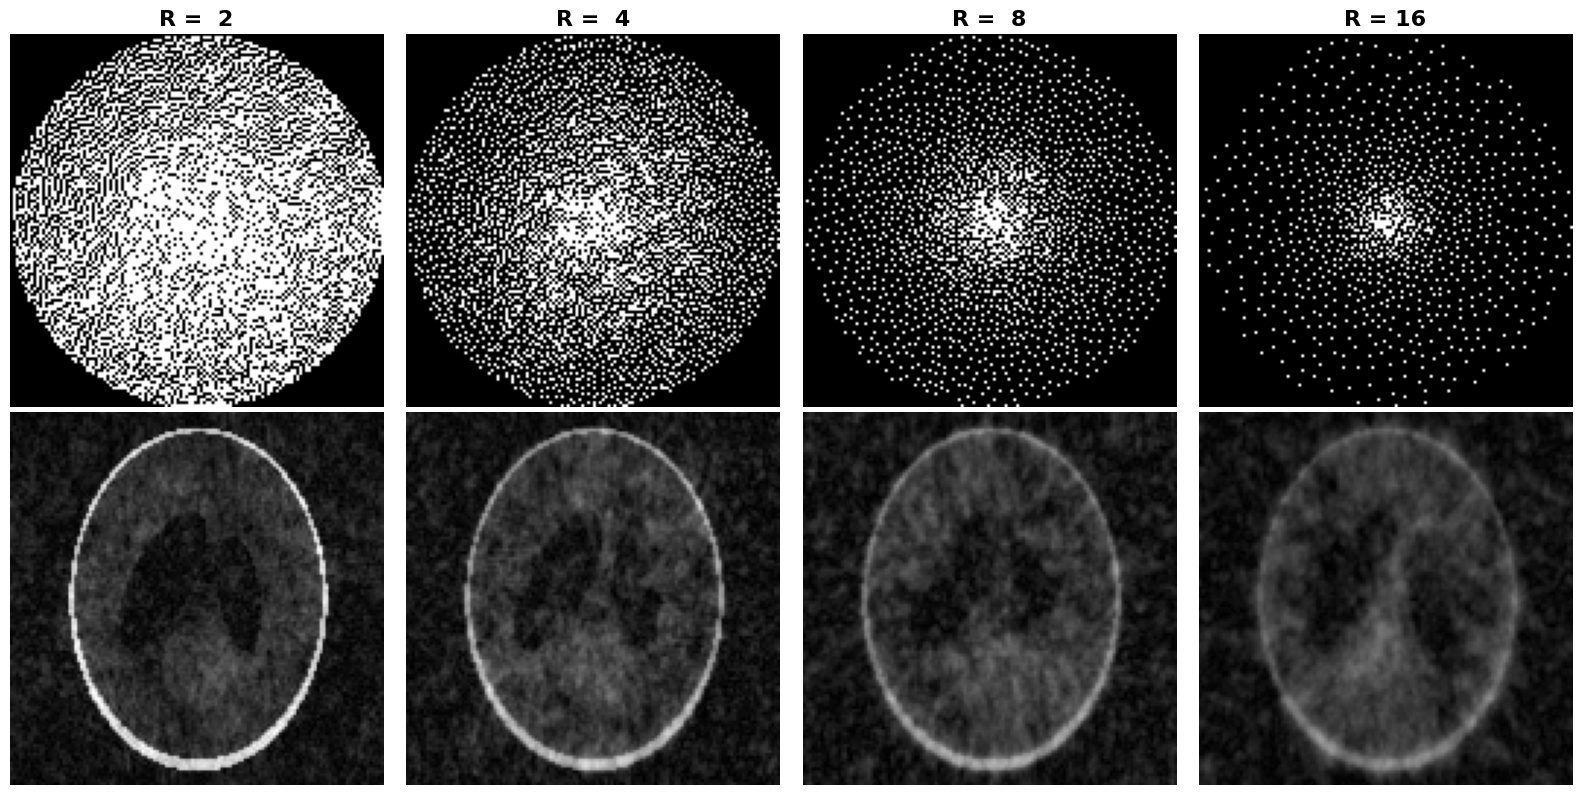
\includegraphics[width=\textwidth]{figures/usamp_poisson.png}
		\end{figure}
	\end{frame}
	
	\begin{frame}{Non-Uniform Undersampling: Radial}
		\begin{figure}
			\centering
			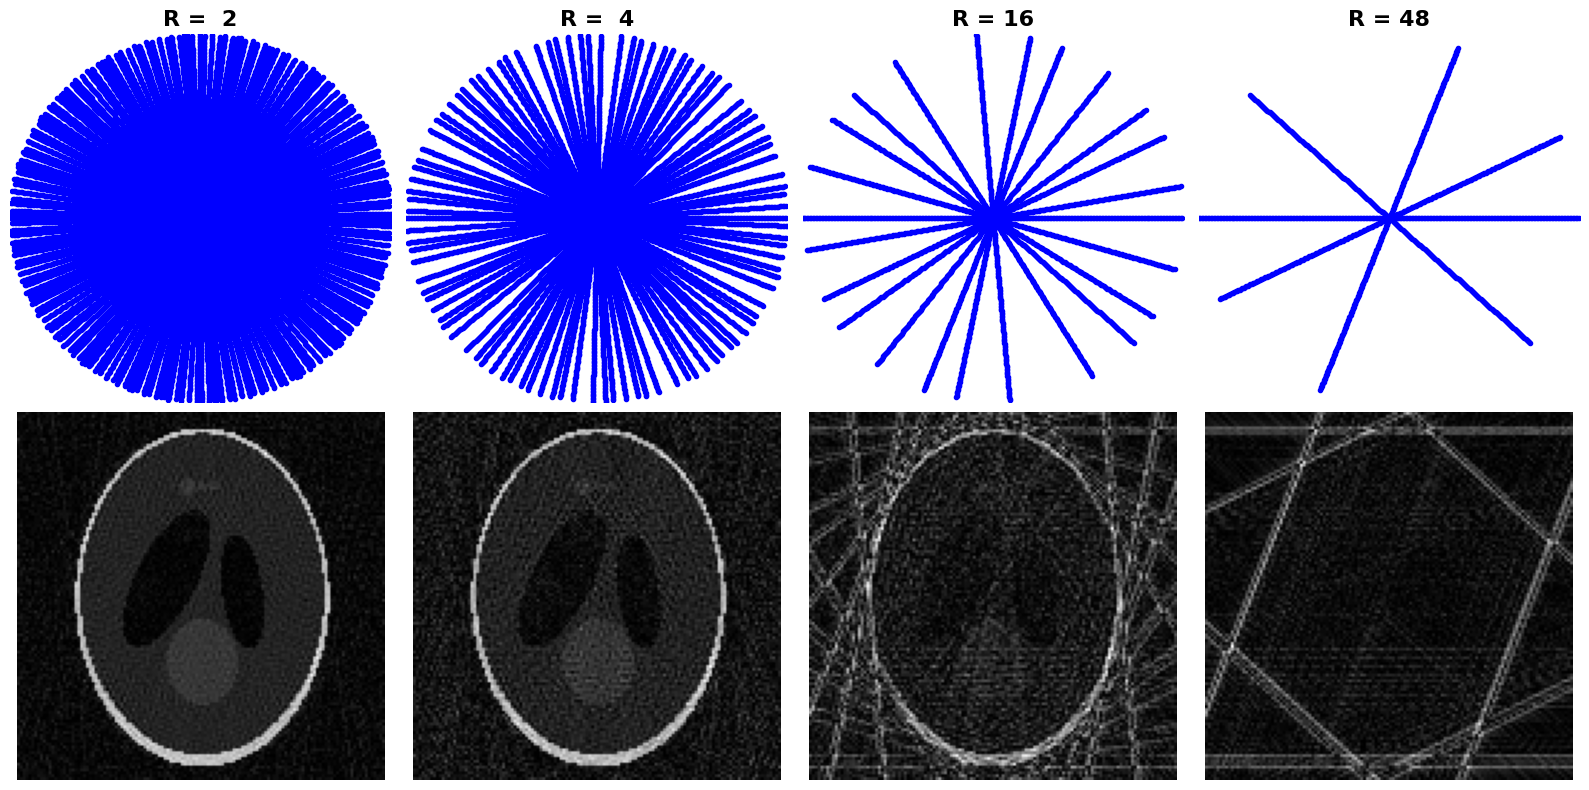
\includegraphics[width=\textwidth]{figures/usamp_radial.png}
		\end{figure}
	\end{frame}
	
	\begin{frame}{Non-Uniform Undersampling: Spiral}
		\begin{figure}
			\centering
			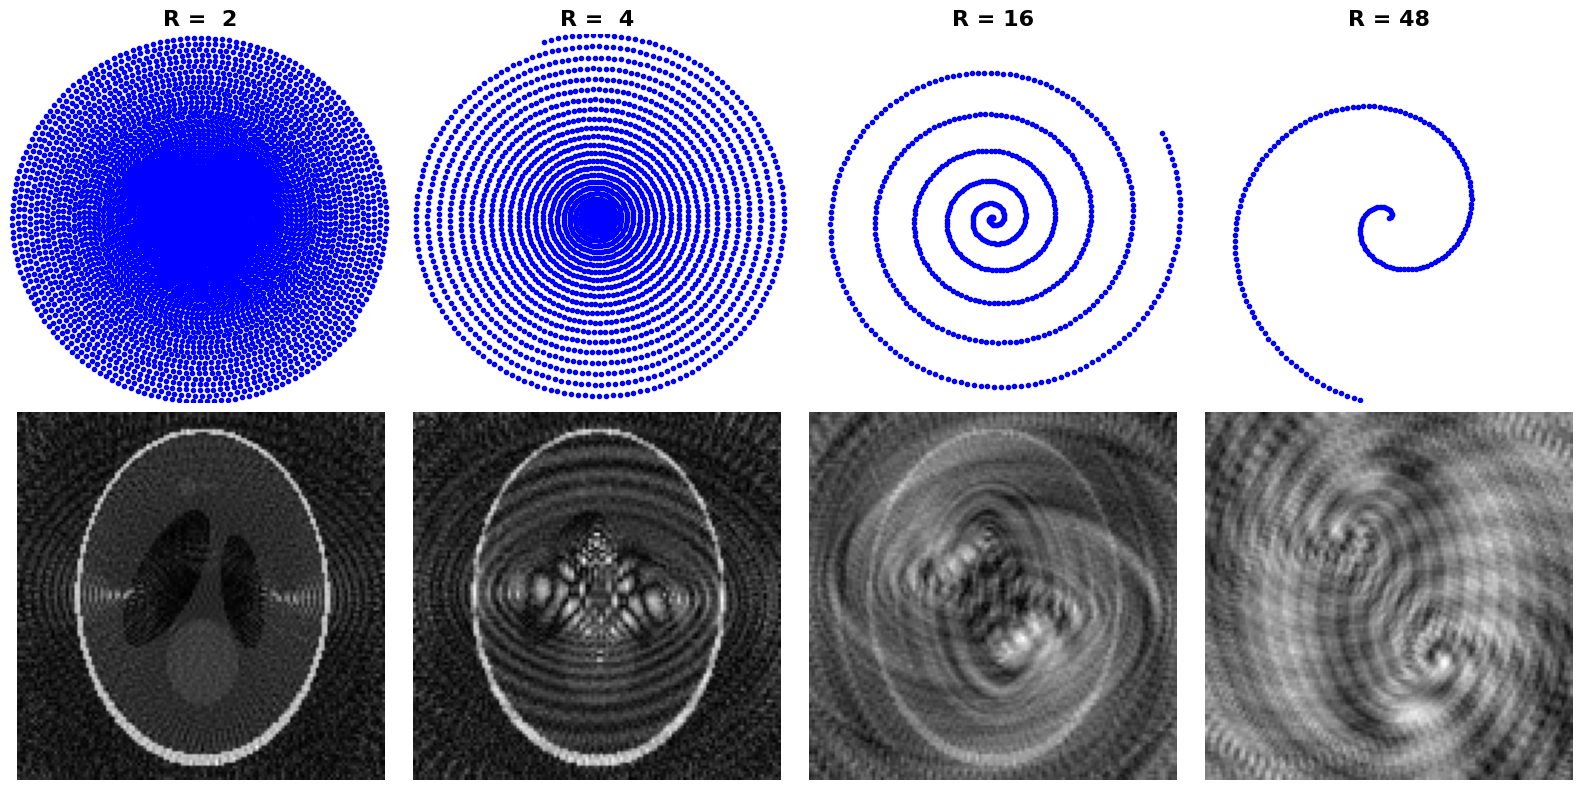
\includegraphics[width=\textwidth]{figures/usamp_spiral.png}
		\end{figure}
	\end{frame}
	
	\begin{frame}{Understand Incoherence via Point Spread Function (PSF)}
		\begin{itemize}
			\item the response of a focused optical imaging system to a point source or point object
			\item the impulse response function of a focused optical imaging system
		\end{itemize}
		
		\begin{figure}
			\centering
			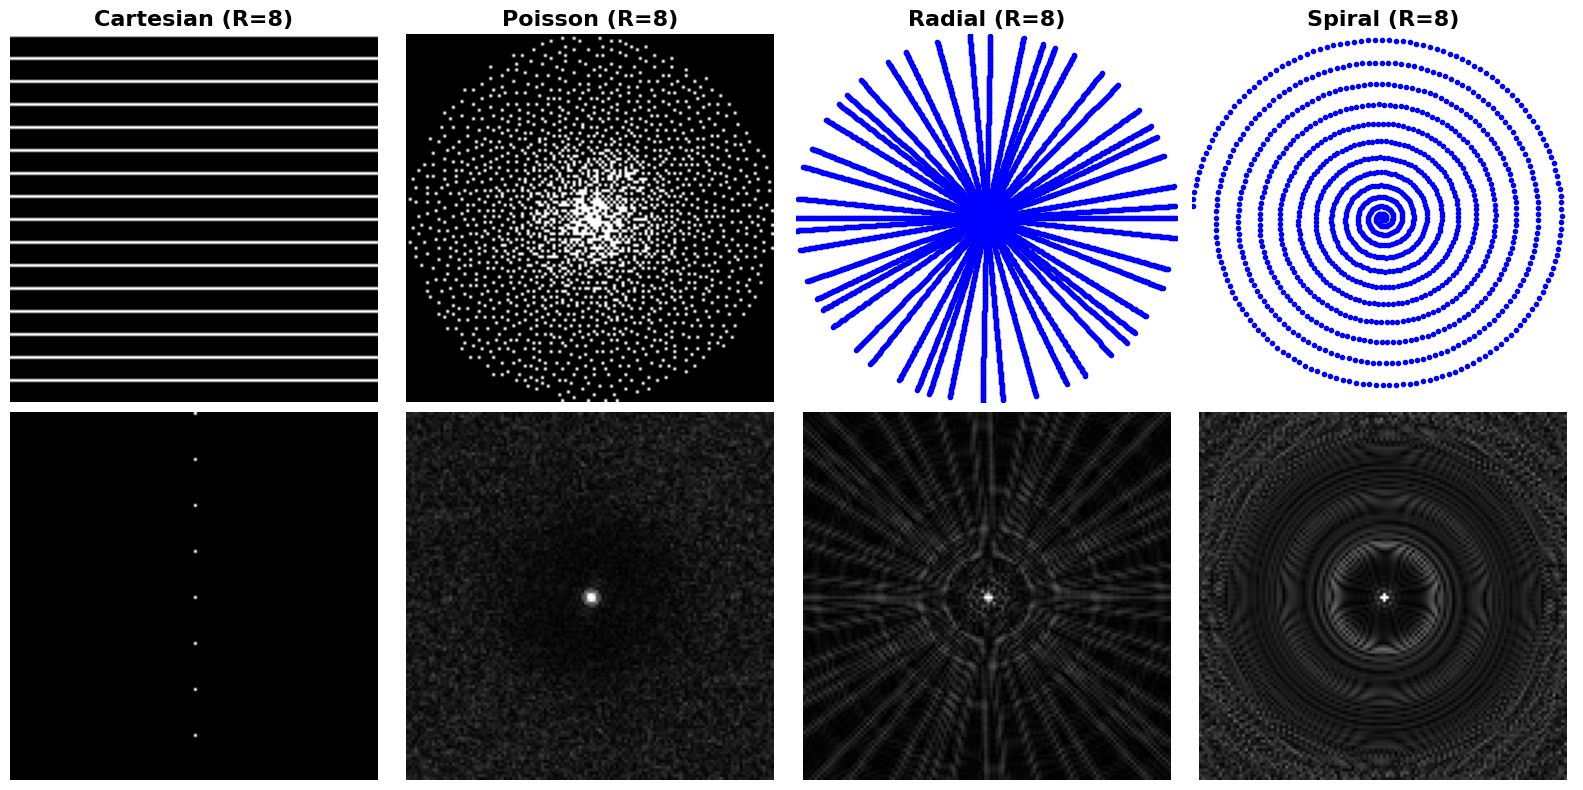
\includegraphics[width=0.95\textwidth]{figures/usamp_psf.png}
		\end{figure}
	\end{frame}
	
	\begin{frame}{Non-Linear Reconstruction}
		\begin{enumerate}
			\item $\ell_1$ regularization with soft thresholding for linear inverse problem 
				\begin{itemize}
					\item Beck A, Teboulle M. A fast iterative shrinkage-thresholding algorithm for linear inverse problems. \textit{SIAM J Imaging Sciences} (2009).
				\end{itemize}
			
			\vspace{1em}
			\item Non-linear model-based reconstruction 
				\begin{itemize}
					\item Block KT, Uecker M, Frahm J. Model-based iterative reconstruction for radial fast spin-echo MRI. \textit{IEEE Trans Med Imaging} (2009).
					\item Fessler JA. Model-based image reconstruction for MRI. \textit{IEEE Signal Process Mag} (2010).
					\item Doneva M, B\"ornert P, Eggers H, Stehning C, S\'en\'egas J, Mertins A. Compressed sensing reconstruction for magnetic resonance parameter mapping. \textit{Magn Reson Med} (2010).
					\item Ma D, Gulani V, Seiberlich N, et al. Magnetic resonance fingerprinting. \textit{Nature} (2013).
				\end{itemize}
		\end{enumerate}
	\end{frame}
	
	\begin{frame}{Let's Begin with Parallel Imaging as Linear Inverse Problem}
		\begin{figure}
			\centering
			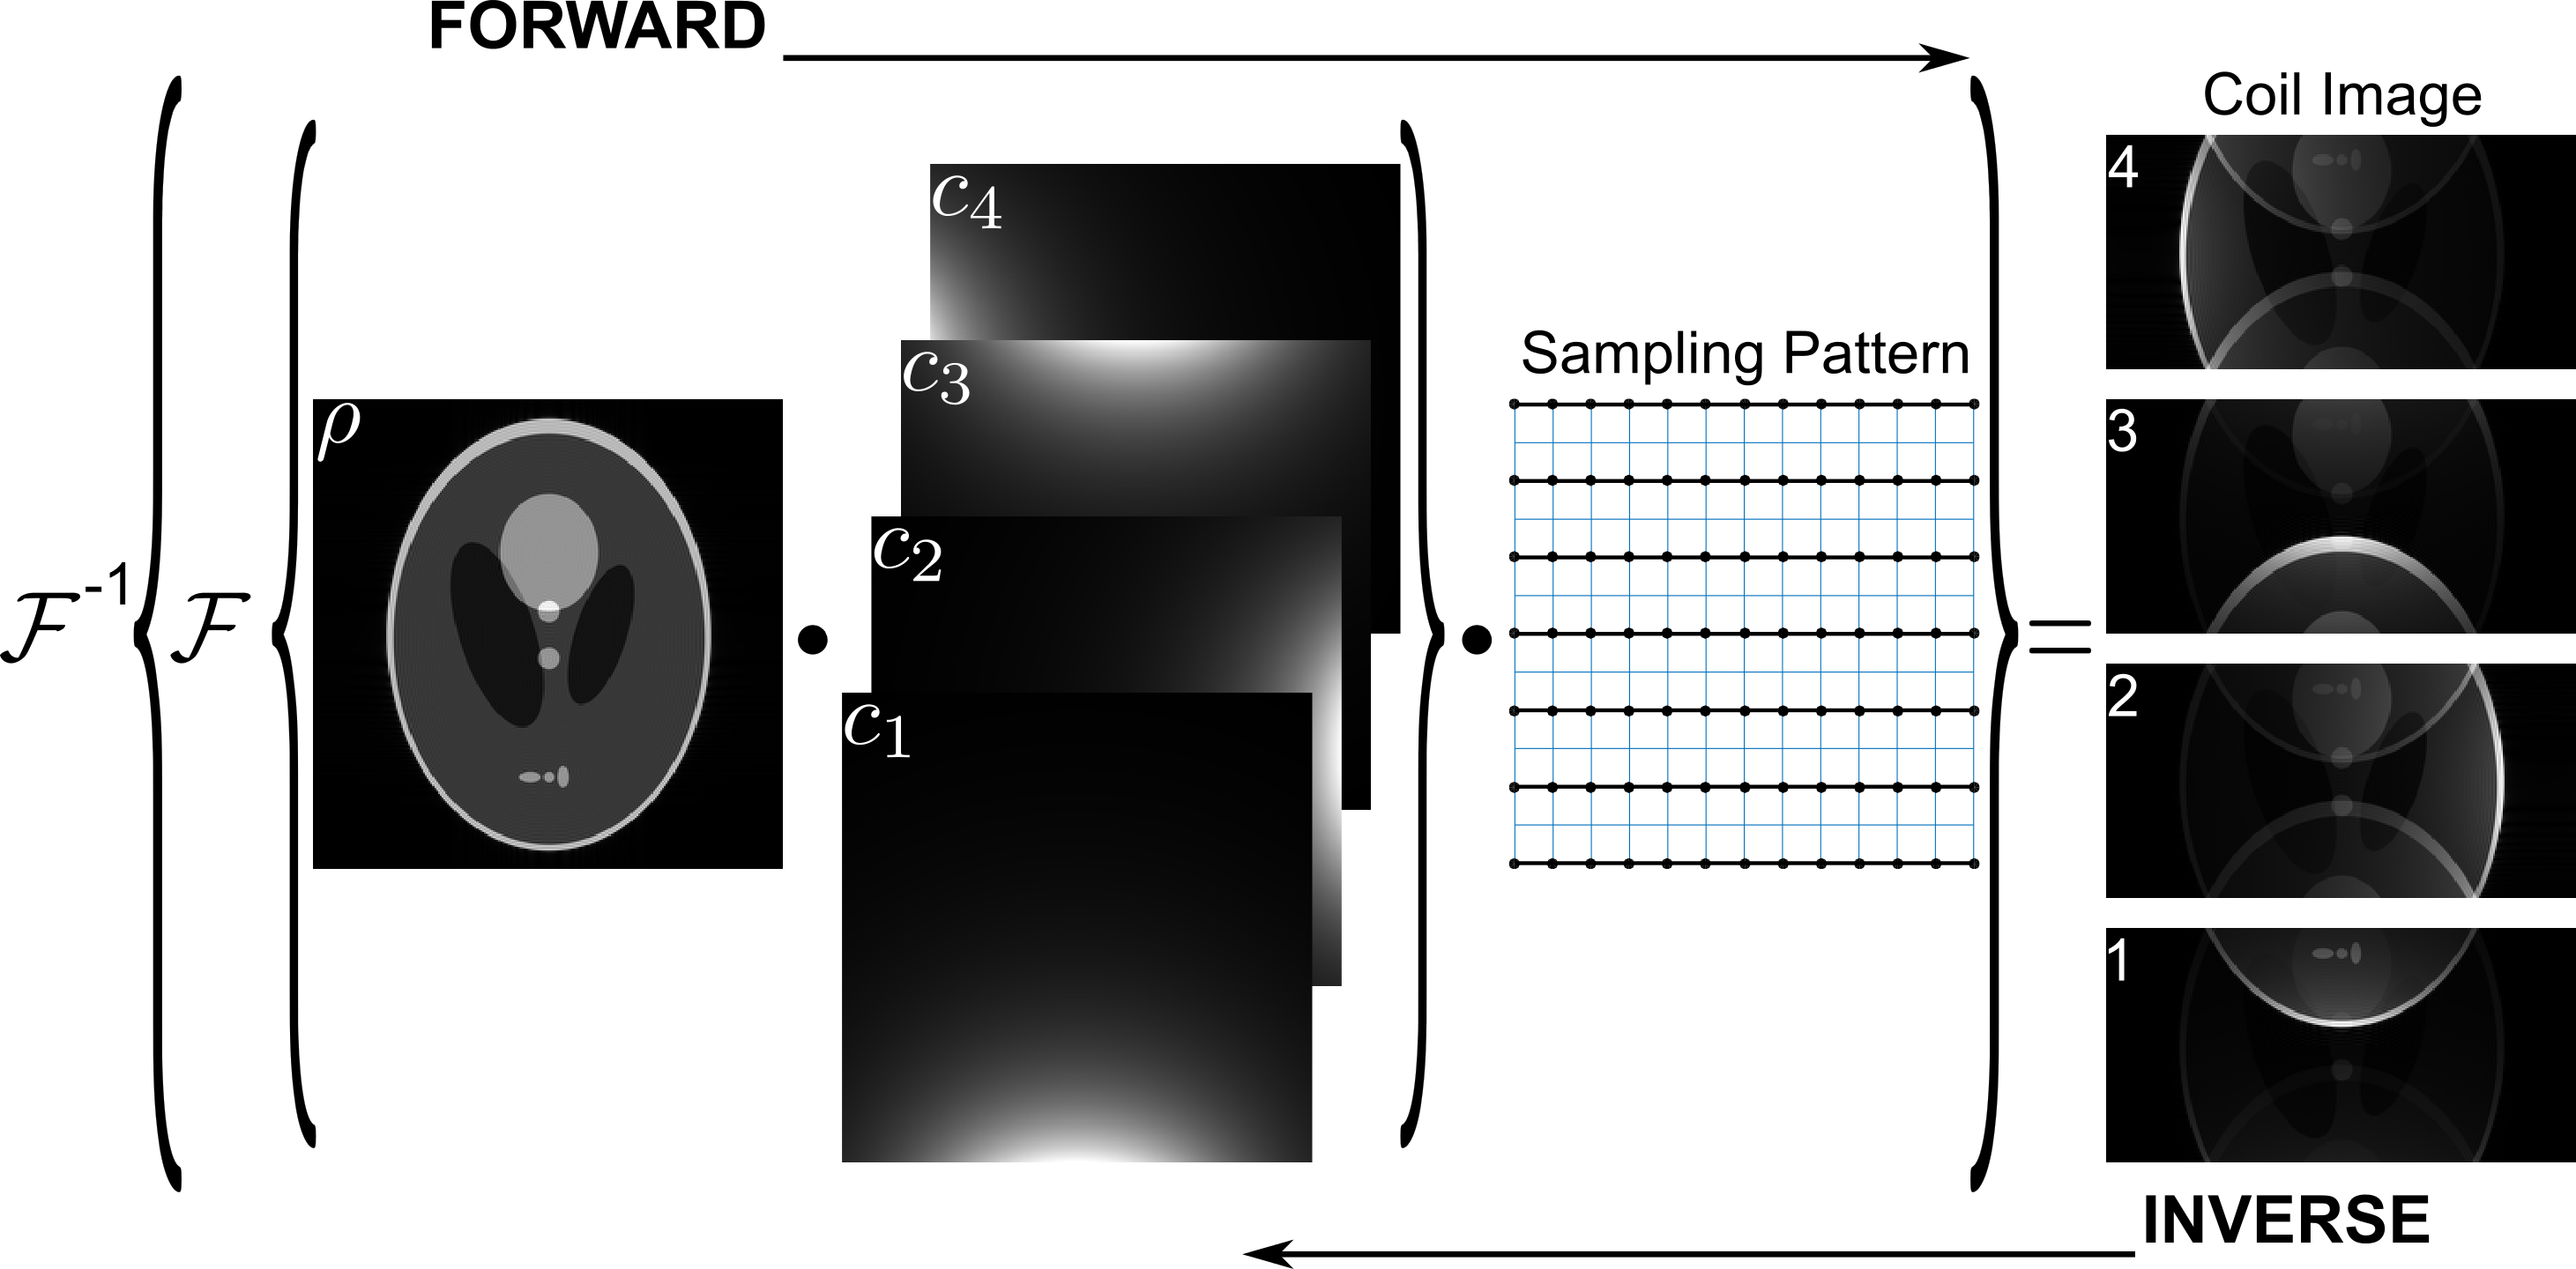
\includegraphics[width=0.8\textwidth]{figures/mri-pi.png}
		\end{figure}
		
		\begin{equation}
			\argmin_x \norm{y - \mathbf{P} \mathbf{F} \mathbf{C} x}_2 + \lambda \norm{x}_2
		\end{equation}
	\end{frame}
	
	\begin{frame}{Solution}
		\begin{itemize}
			\item Gradient update rule:
			
			\begin{equation}
				x^{(k+1)} = x^{(k)} - \alpha \mathbf{C}^* \mathbf{F}^{-1} \mathbf{P}^* (y - \mathbf{P}\mathbf{F}\mathbf{C}x^{(k)})
			\end{equation}
			
			\vspace{1em}
			\item Can be solved efficiently by gradient descent, conjugate gradient, ...
		\end{itemize}
	\end{frame}
	
	\begin{frame}{Sparsity Constraint}
		\begin{equation}
			\argmin_x \norm{y - \mathbf{P} \mathbf{F} \mathbf{C} x}_2 + \lambda \norm{\mathbf{R}x}_1
		\end{equation}
		
		\begin{itemize}
			\item $\ell_1$ function is not differentiable
		\end{itemize}
		\begin{figure}
			\centering
			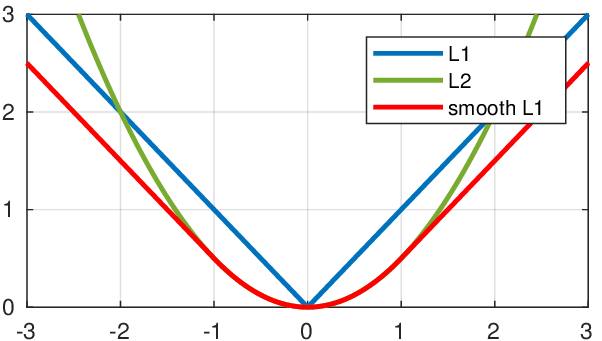
\includegraphics[width=0.55\textwidth]{figures/l1-l2-plots.png}
			\captionsetup{labelformat=empty}
			\caption{{\tiny Feng ZH, Kittler J, Awais M, Huber P. Wing loss for robust facial landmark localisation with CNN. \textit{CVPR} (2018).}}
		\end{figure}
	\end{frame}
	
	\begin{frame}{Fast Iterative Soft Thresholding (FISTA)}
		\begin{figure}
			\centering
			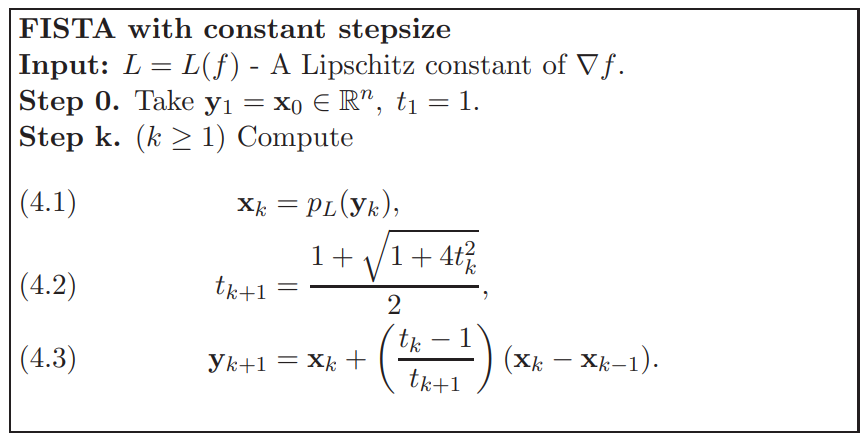
\includegraphics[width=0.7\textwidth]{figures/fista.png}
		\end{figure}
	
		\begin{itemize}
			\item the function $p$ is defined as:
			\begin{align}
				x^{(k+1)} &= \mathcal{T}_{\lambda \alpha} (x^{(k)} - \alpha \mathbf{A}^T (\mathbf{A} x^{(k)} - b)) \\
				\mathcal{T}_c &= (|x| - c)_{+} \text{sgn}(x)
			\end{align}
		\end{itemize}
	\end{frame}
	
	\begin{frame}{Toy Example}
		\begin{figure}
			\centering
			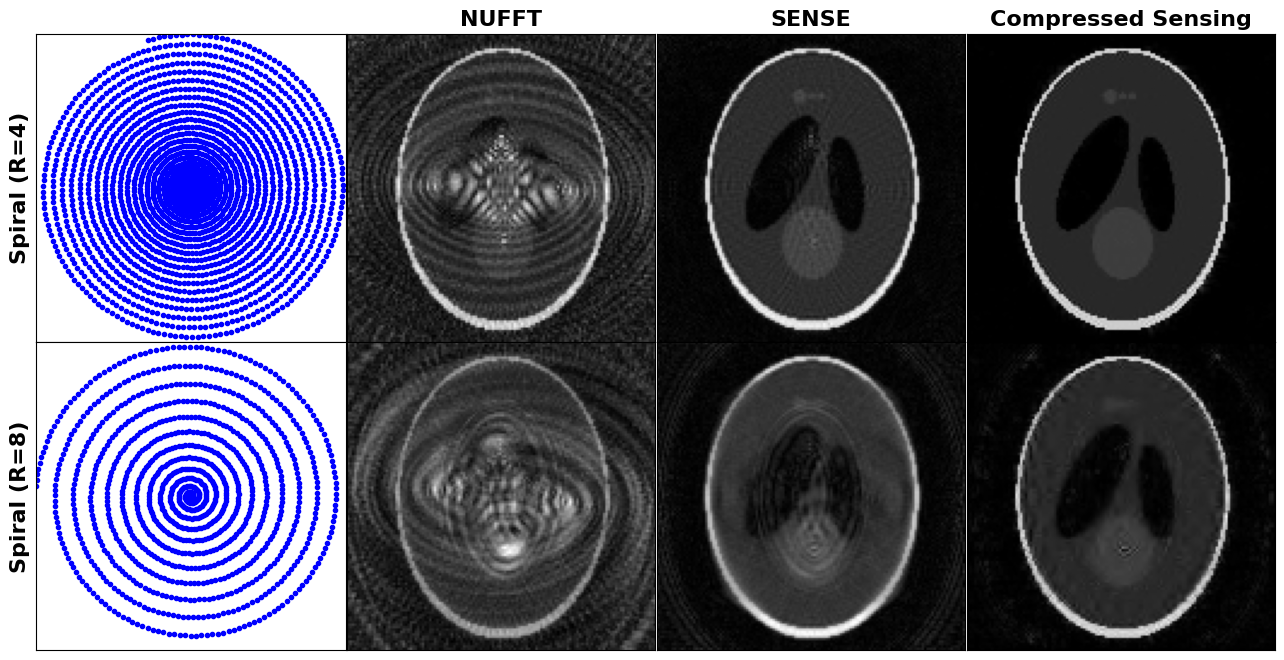
\includegraphics[width=\textwidth]{figures/phan_recon.png}
		\end{figure}
	\end{frame}
	
	\begin{frame}{Beyond 2D: $k$-$t$ Sparsity \footnote{Lustig M, Santos JM, Donoho DL, Pauly JM. k-t SPARSE: High frame rate dynamic MRI exploiting spatio-temporal sparsity. \textit{ISMRM} (2006).}}
		\begin{figure}
			\centering
			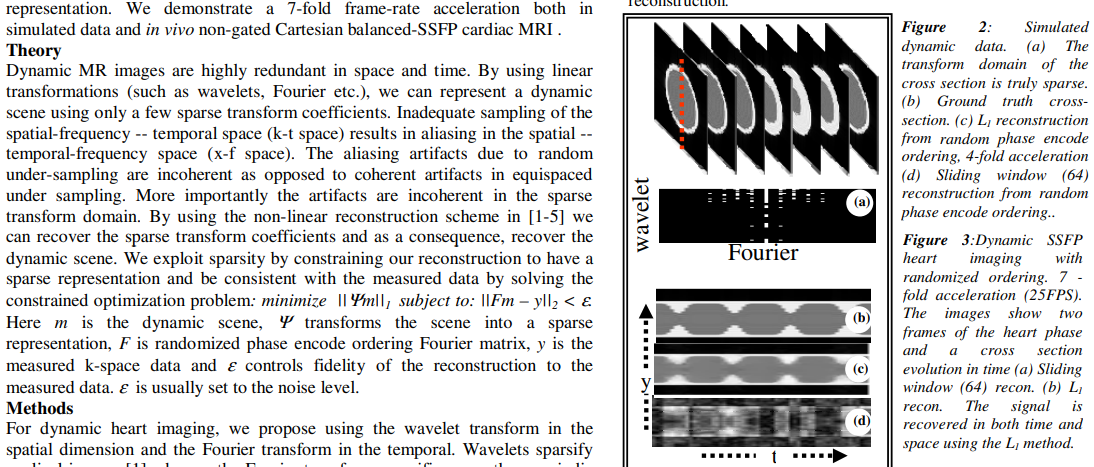
\includegraphics[width=\textwidth]{figures/k-t_sparse.png}
		\end{figure}
	\end{frame}
	
	\begin{frame}{Non-Linear Model-Based Reconstruction}
		\begin{itemize}
			\item <1-> From parallel imaging to high-dimensional imaging
			
			\item <2-> Can we \underline{chain} the Bloch equation into the parallel imaging forward model?
			\begin{equation}
				\argmin_x \norm{y - \mathbf{P} \mathbf{F} \mathbf{C} \mathbf{B} x}_2 + \lambda \mathbf{R}(x)
			\end{equation}
			
			\item <3-> Examples of $\mathbf{B}$:
			\begin{align}
				\mathbf{B}(M_0, T_2) &:= M_0 \cdot e^{-t/T_2} \\
				\mathbf{B}(M_\text{ss}, M_0, T_1) &:= M_\text{ss} - (M_\text{ss} + M_0) \cdot e^{-t/T_1^*} \\
				\mathbf{B}(\text{W}, \text{F}, T_2^*, f_{B_0}) &:= (\text{W} + \text{F} \cdot z_t) \cdot e^{-i2\pi f_{B_0} t} \cdot e^{- t/T_2^*} \\
				& \cdots
			\end{align}
		\end{itemize}
	\end{frame}
	
	\begin{frame}{Example: Phase-Contrast Flow}
		\begin{figure}
			\centering
			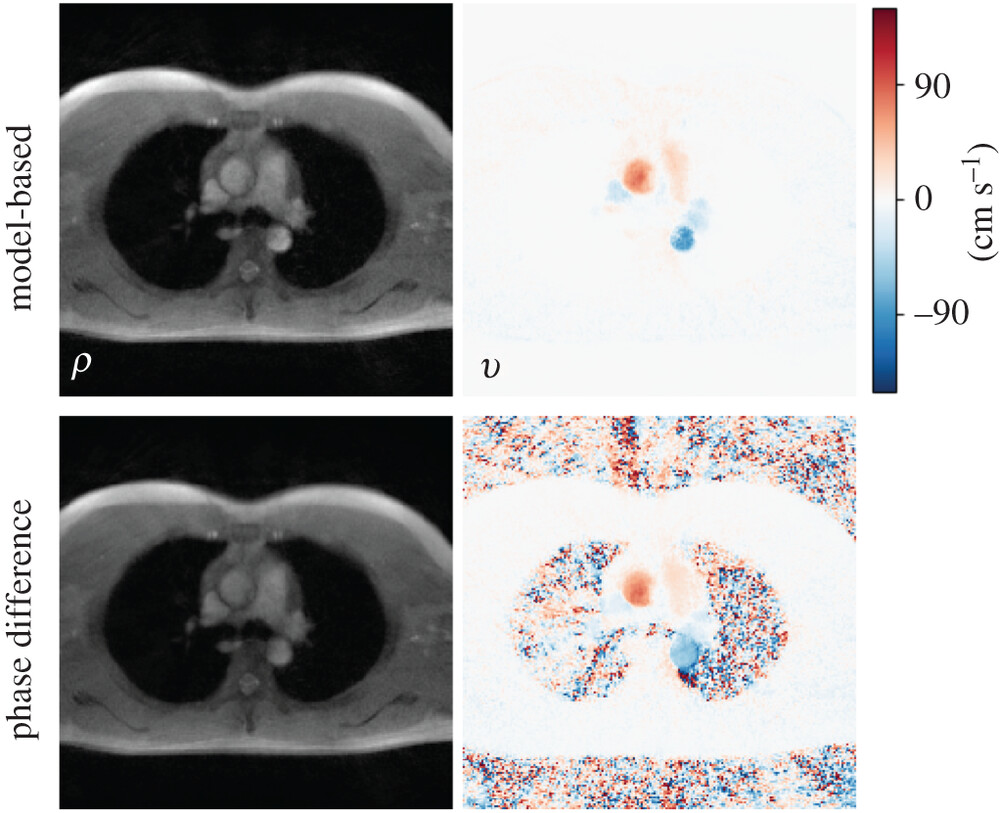
\includegraphics[width=0.65\textwidth]{figures/flow.jpg}
		\end{figure}
	\end{frame}
	
	\begin{frame}{Example: Fat, $T_2^*$, and $B_0$ Field Inhomogeneity}
		\begin{figure}
			\centering
			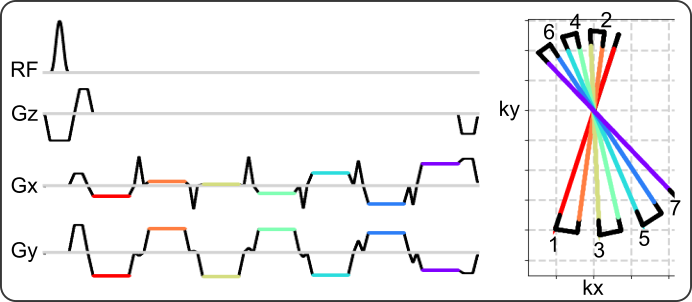
\includegraphics[width=0.6\textwidth]{figures/meco.png}
		\end{figure}
		
		\begin{figure}
			\centering
			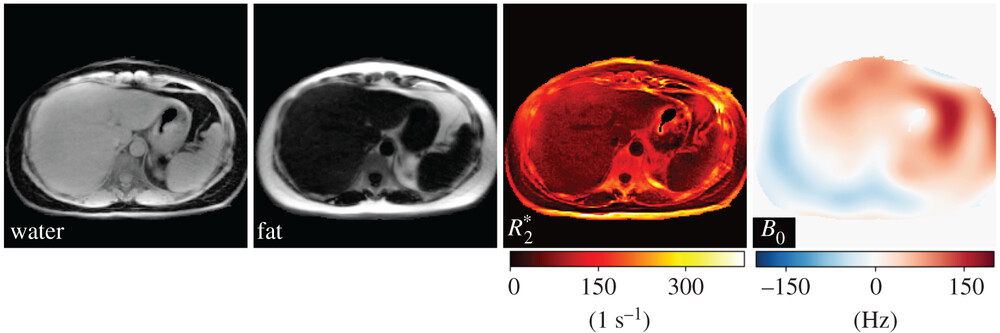
\includegraphics[width=0.8\textwidth]{figures/meco_liver.jpg}
		\end{figure}
	\end{frame}
	
	% ============================================ %
	\section{Low Rank}
	
	\begin{frame}{Matrix Rank \footnote{\url{https://en.wikipedia.org/wiki/Rank_(linear_algebra)}}}
		\begin{itemize}
			\item <1-> In linear algebra, the rank of a matrix is the dimension of the vector space spanned by its columns.
			\begin{figure}
				\centering
				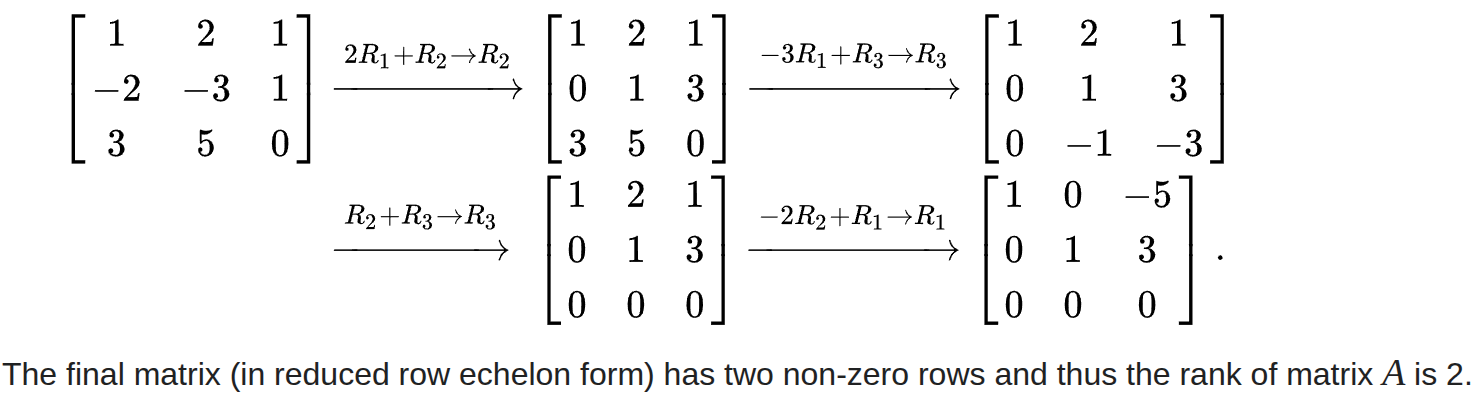
\includegraphics[width=0.8\textwidth]{figures/rank.png}
			\end{figure}

			\vspace{1em}
			\item <2-> Matrix rank can be computed via \underline{singular value decomposition (SVD)}.
		\end{itemize}		
	\end{frame}
	
	\begin{frame}{Spatio-Temporal Imaging}
		\begin{figure}
			\centering
			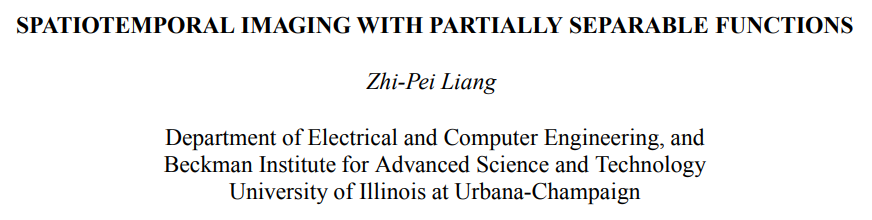
\includegraphics[width=\textwidth]{figures/psf1.png}
		\end{figure}
	\end{frame}
	
	\begin{frame}{Spatio-Temporal Imaging}
		\begin{figure}
			\centering
			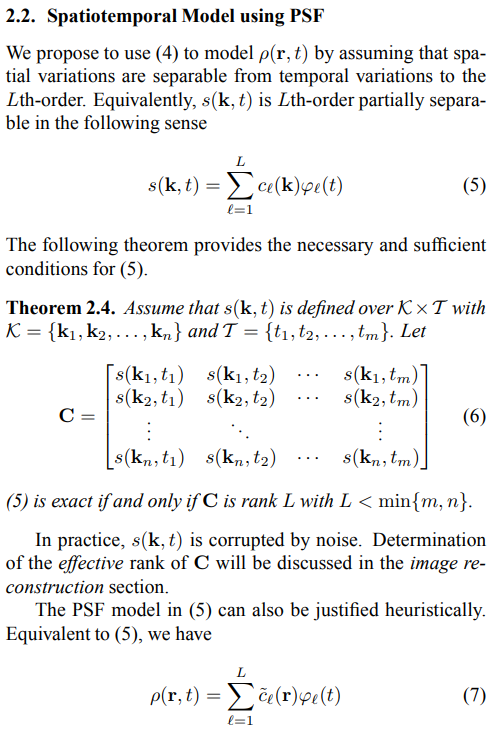
\includegraphics[height=0.85\textheight]{figures/psf2.png}
		\end{figure}
	\end{frame}
	
	\begin{frame}{Toy Example}
		\begin{columns}
			\column{0.3\textwidth}
			\centering
			dynamic image seris
			\vspace{1em}
			\animategraphics[autoplay,loop,height=0.5\textheight]{10}{figures/dyn_phan/frame_}{000}{199}
			
			\column{0.3\textwidth}
			\centering
			spatio-temporal matrix
			\vspace{1em}
			
\includegraphics[height=0.5\textheight]{figures/dyn_phan/spatio-temporal-matrix.png}
			
			\column{0.3\textwidth}
			\centering
			eigenvalues
			\vspace{1em}
			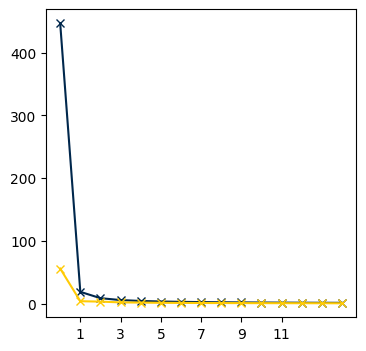
\includegraphics[height=0.5\textheight]{figures/dyn_phan/svd.png}
		\end{columns}
	\end{frame}
	
	\begin{frame}{Locally Low Rank \footnote{Zhang T, Pauly JM, Levesque IR. Accelerating parameter mapping with a locally low rank constraint. \textit{Magn Reson Med} (2015).}}
		\begin{figure}
			\centering
			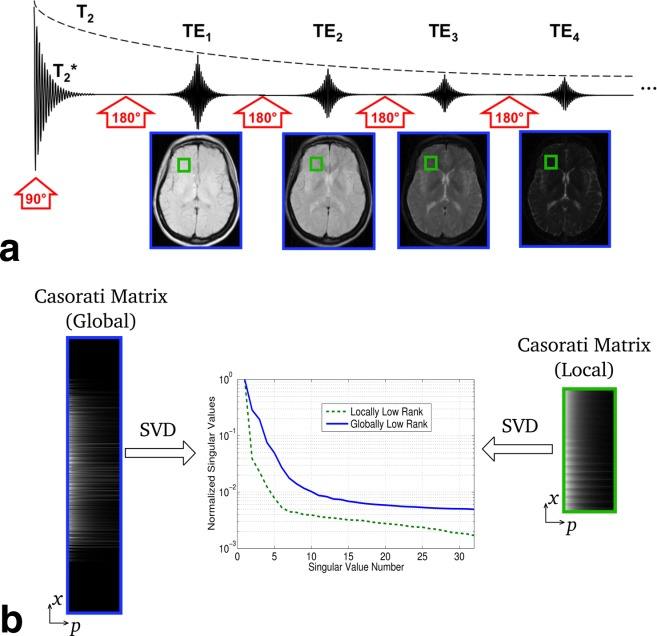
\includegraphics[height=0.8\textheight]{figures/mrm25161-fig-0001-m.jpg}
		\end{figure}
	\end{frame}
	
	\begin{frame}{Low Rank Approximation of Bloch Models \footnote{Huang C, Graff CG, Clarkson EW, Bilgin A, Altbach MI. $T_2$ mapping from highly undersampled data by reconstruction of principle component coefficient maps using compressed sensing. \textit{Magn Reson Med} (2012).}$^,$\footnote{Tamir JI, Uecker M, Chen W, et al. $T_2$ shuffling: sharp, multicontrast, volumetric fast spin-echo imaging. \textit{Magn Reson Med} (2017).}}
		\begin{columns}
			\column{0.4\textwidth}
			\centering
			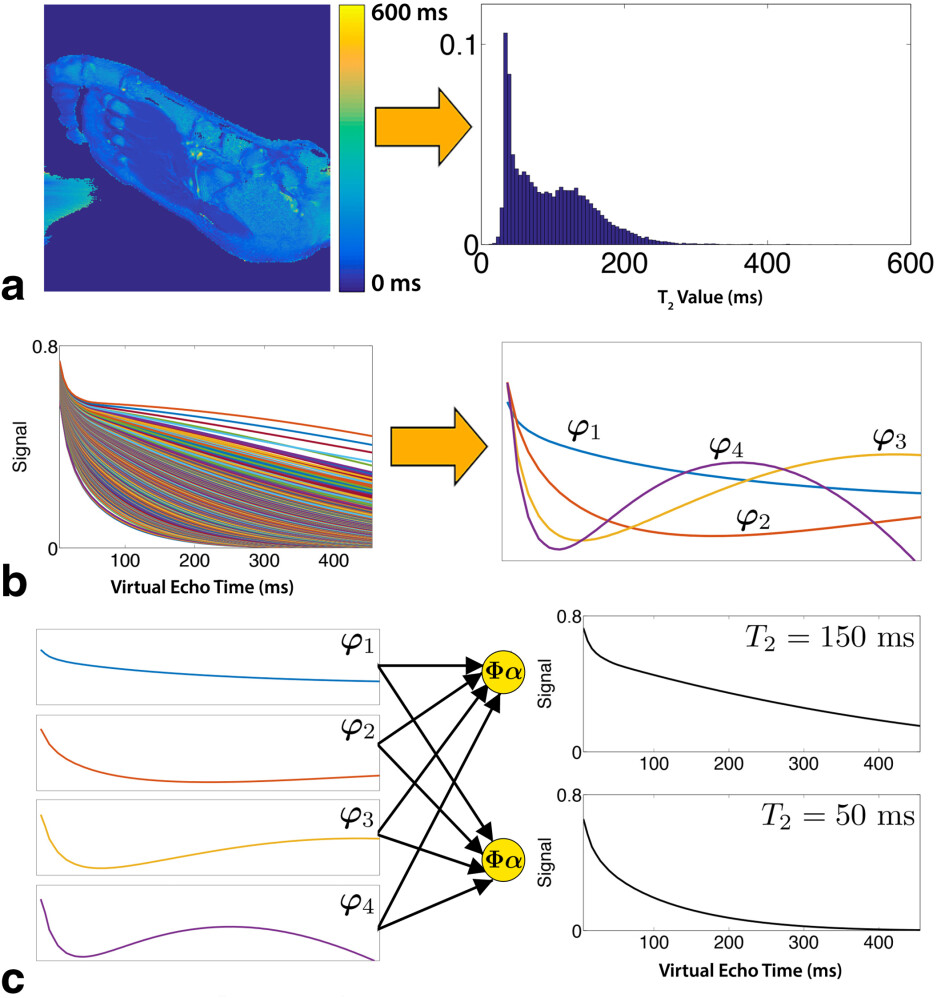
\includegraphics[height=0.75\textheight]{figures/mrm26102-fig-0004-m.jpg}
			
			\column{0.6\textwidth}
			\centering
			\begin{itemize}
				\item <1-> define echo images with the shape $[N_x, N_y, N_t]$
				\begin{equation}
					\rho_t = M_0 \cdot e^{-t / T_2}
				\end{equation}
				
				\item <2-> With low rank approximation
				\begin{align}
					\rho &= \Phi \alpha \\
					\Phi &: [N_t, K] \\
					\alpha &: [N_x, N_y, K]
				\end{align}
				
				\item <3-> $K << N_t$ AND It's a \underline{linear} model!
			\end{itemize}
		\end{columns}
	\end{frame}
	
	\begin{frame}{Low Rank Image Reconstruction}
		\begin{equation}
			\argmin_x \norm{y - \mathbf{P} \mathbf{F} \mathbf{C} \mathbf{\Phi} x}_2 + \lambda \mathbf{R}(x)
		\end{equation}
		
		\begin{figure}
			\centering
			\includegraphics[width=\textwidth]{figures/mrm23128-fig-0002-m.jpg}
		\end{figure}
	\end{frame}
	
	\begin{frame}{Low Rank for Magnetic Resonance Fingerprinting (MRF) \footnote{Zhao B, Setsompop K, Adalsteinsson E, et al. Improved MRF reconstruction with low-rank and subspace modeling. \textit{Magn Reson Med} (2018).}}
		\begin{figure}
			\centering
			\includegraphics[width=0.6\textwidth]{figures/mrm26701-fig-0002-m.jpg}
		\end{figure}
	\end{frame}
	
	\begin{frame}{Structured Low Rank}
		\begin{itemize}
			\item Mapping image series into structured matrices (e.g., Toeplitz or Hankel) to restore the complete image series
			
			\vspace{1em}
			\item MR examples:
			\vspace{0.5em}
			\begin{enumerate}
				\item ESPIRiT: coil calibration; where SENSE meets GRAPPA;
				\vspace{0.5em}
				\item MUSSELS: multi-shot diffusion MRI reconstruciton.
			\end{enumerate}
		\end{itemize}
	\end{frame}
	
	\begin{frame}{ESPIRiT: An eigenvalue approach to autocalibrating parallel MRI}
		\begin{itemize}
			\item Walsh DO, Gmitro AF, Marcellin MW. Adaptive reconstruction of phased array MR imagery. \textit{Magn Reson Med} (2000).
			\vspace{1em}
			
			\item Zhang J, Liu C, Moseley ME. Parallel reconstruction using null operations. \textit{Magn Reson Med} (2011).
			\vspace{1em}
			
			\item Lai P, Lustig M, Brau AC, Vasanawala S, Beatty PJ, Alley M. Efficient L1SPIRiT reconstruction (ESPIRiT) for highly accelerated 3D volumetric MRI with parallel imaging and compressed sensing. \textit{ISMRM} (2010).
			\vspace{1em}
			
			\item Lustig M, Lai P, Murphy M, Vasanawala SS, Elad M, Zhang J, Pauly JM. An eigen-vector approach to autocalibrating parallel MRI, where SENSE meets GRAPPA. \textit{ISMRM} (2011).
			\vspace{1em}
			
			\item Uecker M, Lai P, Murphy MJ, et al. \href{https://doi.org/10.1002/mrm.24751}{ESPIRiT - an eigenvalue approach to autocalibrating parallel MRI: where SENSE meets GRAPPA}. \textit{Magn Reson Med} (2014).
		\end{itemize}
	\end{frame}
	
	\begin{frame}{ESPIRiT}
		\begin{figure}
			\centering
			\includegraphics[width=0.85\textwidth]{figures/mrm24751-fig-0002-m.jpg}
		\end{figure}
	\end{frame}
	
	\begin{frame}{ESPIRiT}
		\begin{figure}
			\centering
			\includegraphics[width=0.85\textwidth]{figures/mrm24751-fig-0003-m.jpg}
		\end{figure}
	\end{frame}
	
	\begin{frame}{ESPIRiT}
		\begin{figure}
			\centering
			\includegraphics[width=0.85\textwidth]{figures/mrm24751-fig-0004-m.jpg}
		\end{figure}
	\end{frame}
	
	\begin{frame}{Example: ESPIRiT on \underline{Reduced FOV} Imaging}
		\begin{columns}
			\column{0.7\textwidth}
			\begin{figure}
				\centering
				\includegraphics[width=\columnwidth]{figures/espirit_coil_images.png}
			\end{figure}
			
			\column{0.3\textwidth}
			\begin{figure}
				\centering
				\includegraphics[width=\columnwidth]{figures/espirit_rss.png}
			\end{figure}
			
			\centering
			$\text{RSS} : \sqrt{\sum_i (c_i \cdot \rho)^2}$
		\end{columns}
	\end{frame}

	\begin{frame}{Step \#1: Retrospective Undersampling}
		\begin{columns}
			\column{0.7\textwidth}
			\begin{figure}
				\centering
				\includegraphics[width=\columnwidth]{figures/espirit_undersampled_kspace.png}
			\end{figure}
			
			\column{0.3\textwidth}
			\begin{figure}
				\centering
				\includegraphics[width=\columnwidth]{figures/espirit_zf.png}
			\end{figure}
		\end{columns}
		
		Curious about the black space on the left and the right sides of k-space?
		\begin{itemize}
			\item [$\rightarrow$] Shimron E, Tamir JI, Wang K, Lustig M. Implicit data crimes: machine learning bias arising from misuue of public data. \textit{Proc Natl Acad Sci U.S.A.} (2022).
		\end{itemize}
	\end{frame}

	\begin{frame}{Step \#2: ESPIRiT with 1 Set of Coil Sensitivity Maps}
		\begin{figure}
			\centering
			\includegraphics[width=\textwidth]{figures/espirit_coil1.png}
		\end{figure}
	\end{frame}
	
	\begin{frame}{Step \#3: SENSE Reconstruction}
		\begin{equation}
			\argmin_x \norm{y - \mathbf{P} \mathbf{F} \mathbf{C} x}_2 + \lambda \norm{x}_2 \; \text{with} \; x \in \mathbb{C}^{N_x \times N_y}
		\end{equation}
		
		\begin{figure}
			\centering
			\includegraphics[height=0.75\textheight]{figures/espirit_sense1.png}
		\end{figure}
	\end{frame}
	
	\begin{frame}{Step \#4: ESPIRiT with 2 Sets of Coil Sensitivity Maps}
		\begin{figure}
			\centering
			\includegraphics[width=\textwidth]{figures/espirit_coil2.png}
		\end{figure}
	\end{frame}
	
	\begin{frame}{Step \#5: Soft SENSE Reconstruction}
		\begin{equation}
			\argmin_x \norm{y - \mathbf{P} \mathbf{F} \sum_{j=1}^2 (\mathbf{C}_j x_j)}_2 + \lambda \norm{x}_2 \; \text{with} \; x \in \mathbb{C}^{N_x \times N_y \times 2}
		\end{equation}
		
		\begin{figure}
			\centering
			\includegraphics[height=0.80\textheight]{figures/espirit_sense2.png}
		\end{figure}
	\end{frame}
	
	\begin{frame}{MUSSELS}
		\begin{figure}
			\centering
			\includegraphics[width=\textwidth]{figures/mrm26382-fig-0001-m.jpg}
		\end{figure}
	\end{frame}

	\begin{frame}{MUSSELS}
		\begin{figure}
			\centering
			\includegraphics[width=\textwidth]{figures/mrm26382-fig-0002-m.jpg}
		\end{figure}
	\end{frame}
	
	\begin{frame}{Comparing LLR and MUSSELS for Multi-Shot EPI \footnote{\url{https://doi.org/10.1162/imag_a_00085}}}
		\begin{figure}
			\centering
			\includegraphics[width=0.95\textwidth]{figures/imag_a_00085_fig4.png}
		\end{figure}
	\end{frame}
	
	\begin{frame}{Beyond Low Rank: 0.7 mm Isotropic Diffusion MRI}
		\begin{figure}
			\centering
			\includegraphics[width=0.75\textwidth]{figures/deepdwi_fig8.png}
		\end{figure}
	\end{frame}
	
	\begin{frame}{Questions}
		\begin{enumerate}
			\item <1-> Why are images from Poisson sampling so blurry?
			
			\vspace{1em}
			\item <2-> Given that MR images are complex-valued, how is soft thresholding performed?
			
			\vspace{1em}
			\item <3-> A dictionary is required to "learn" the subspace matrix $\Phi$, what defines the shape of the dictionary?
		\end{enumerate}
	\end{frame}
	
	\begin{frame}{Beyond Compressed Sensing: What do you spot in this figure?}
		\begin{figure}
			\centering
			\includegraphics[width=0.8\textwidth]{figures/41598_2020_70551_Fig2_HTML.png}
		\end{figure}
	\end{frame}
	
	\begin{frame}{Summary}
		
		\begin{itemize}
			\item <1-> Compressed sensing:
			\begin{enumerate}
				\vspace{0.5em}
				\item incoherent sampling;
				\vspace{0.5em}
				\item sparsity $\ell1$ constraint.
			\end{enumerate}
			
			\vspace{1em}
			\item <2-> Low rank:
			\begin{enumerate}
				\vspace{0.5em}
				\item representation of high-dimensional data in low dimension;
				\vspace{0.5em}
				\item beneficial to multi-contrast, dynamic imaging.
			\end{enumerate}
			
			\vspace{1em}
			\item <3-> {\textcolor{blue}{If you are interested in the topics and look for research projects, reach out \href{mailto:zgtan@umich.edu}{zgtan@umich.edu}}}
		
		\end{itemize}
	\end{frame}
	
	
	
\end{document}